\author{Tadd\"aus Nauheimer}
\chapter{Step-by-Step Guide}

\section{How To}
Um die Software aufzurufen einfach auf die Ihnen bereitgestellte URL gehen.
Darauf kann diesem Guide gefolgt werden.

\subsection{Frontpage und Dokument laden}

Hier ist die Frontpage der Software zu sehen, oben Links kann das erste Dokument geladen werden.
Zu beachten hier ist, dass dies ein etweder leeres Dokument sein sollte oder eine korrekt ausgef\"ullte Mussterl\"osung

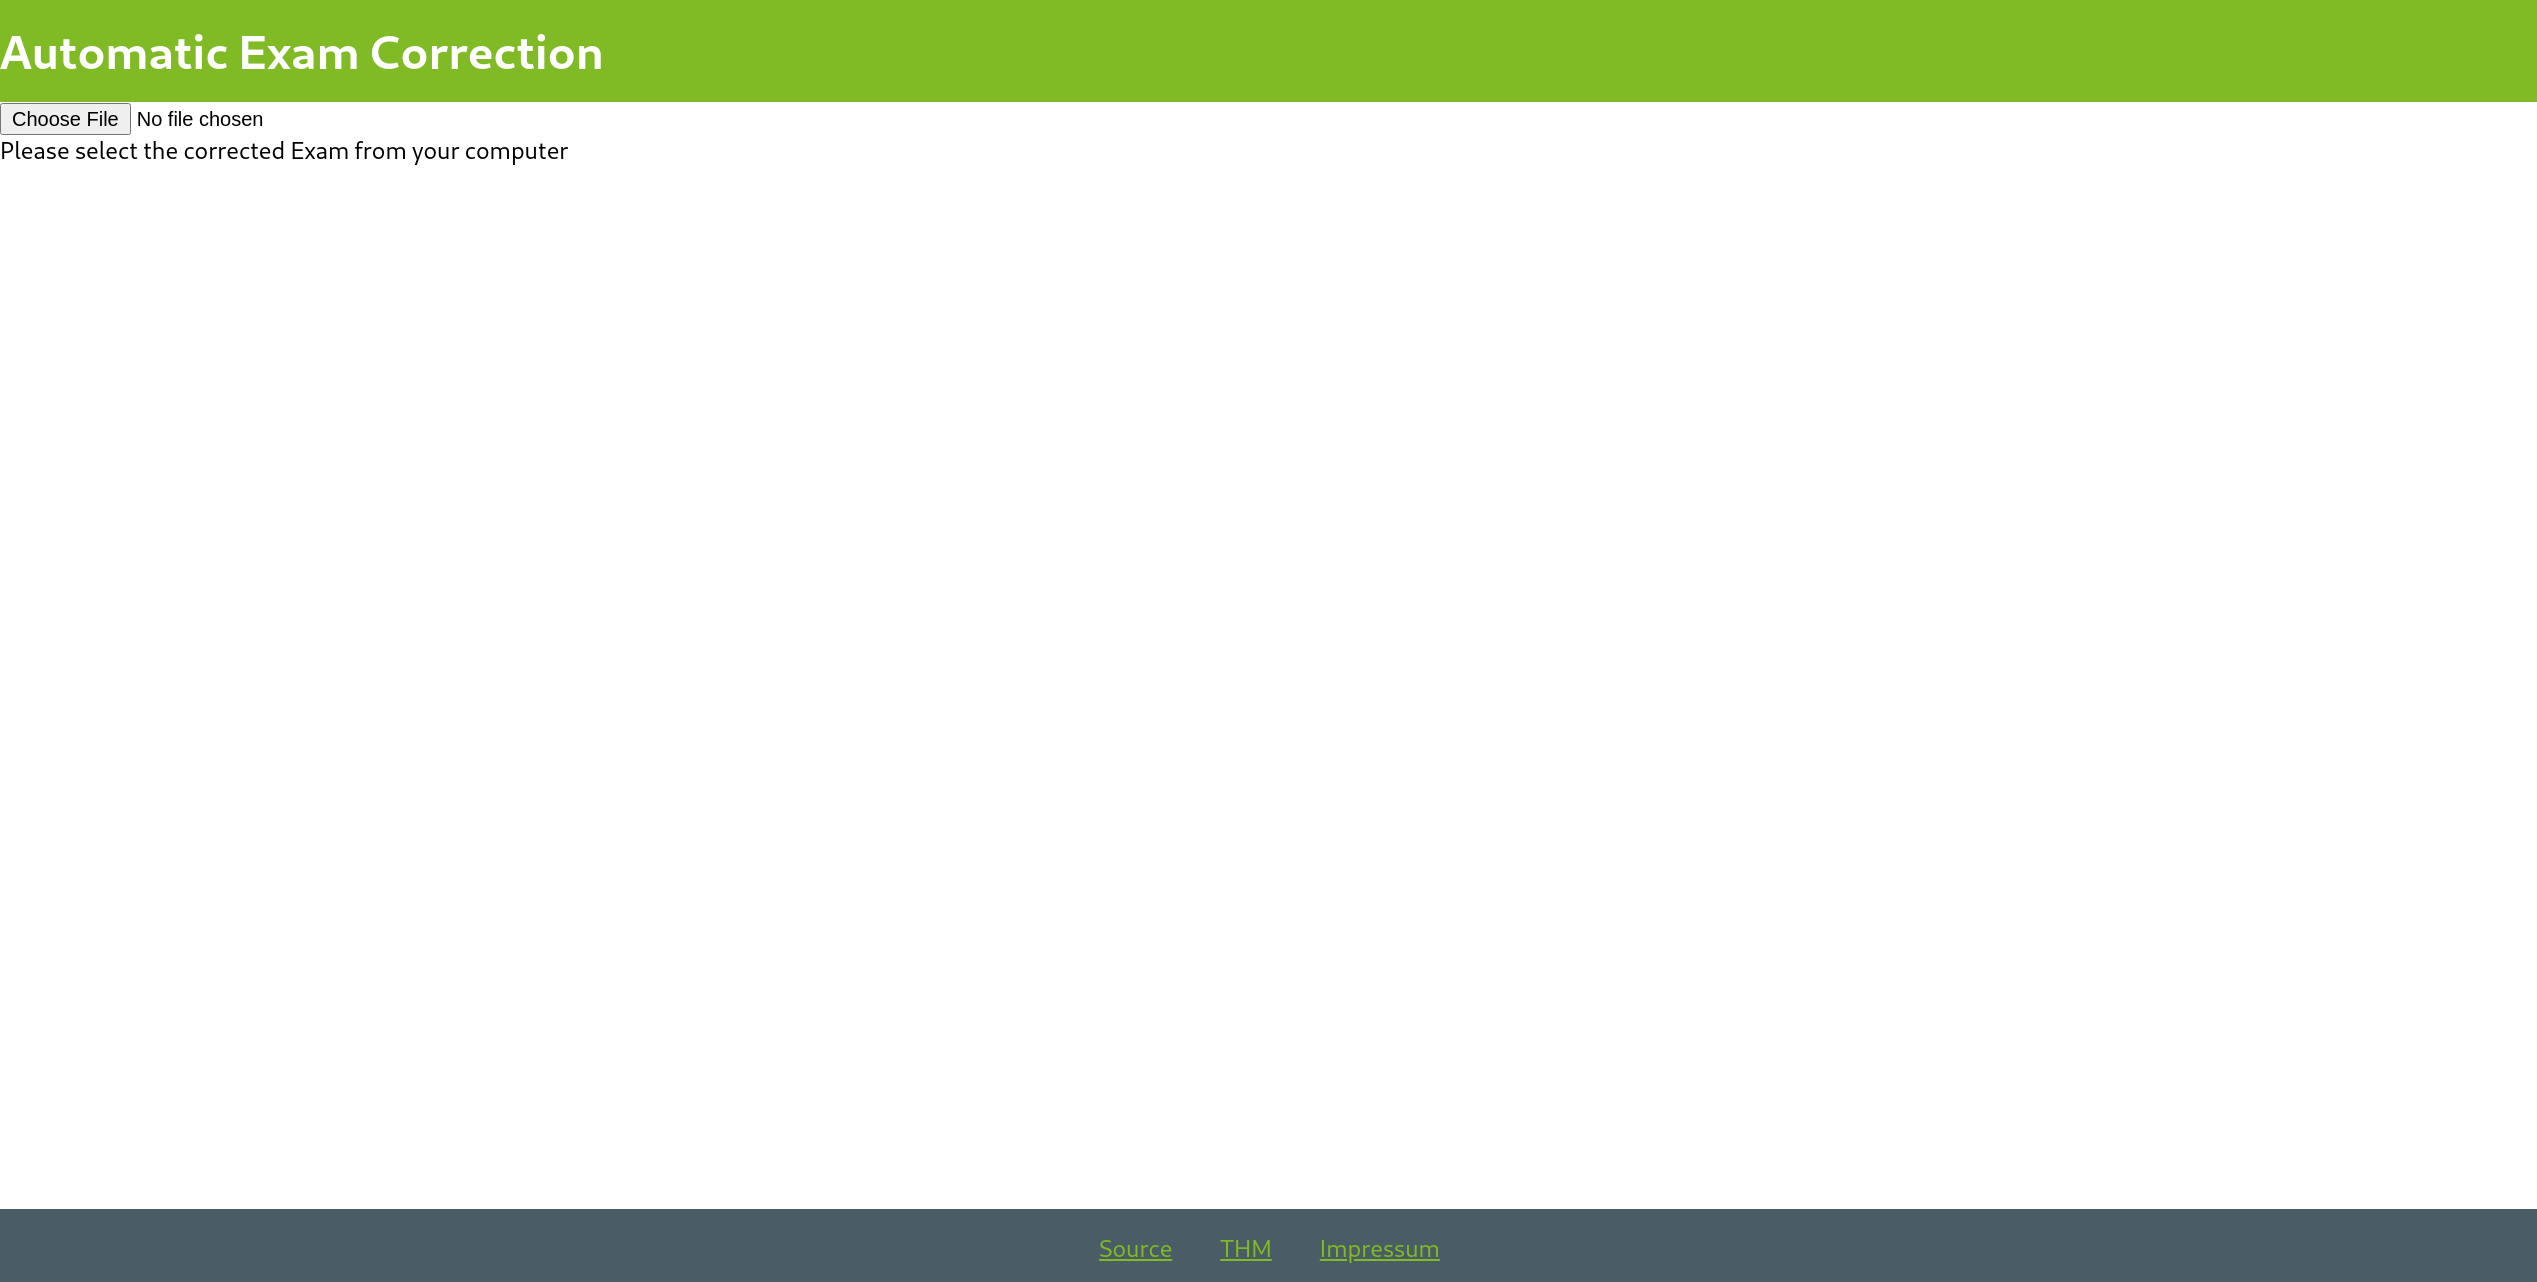
\includegraphics[width=\textwidth]{frontpage-view}

\subsection{Aufgaben Ausw\"ahlten}

Sobalt dieses Dokument geladen ist, sieht man diese Seite. 
Ab hier kann begonnen werden Aufgaben auszuw\"ahlen.

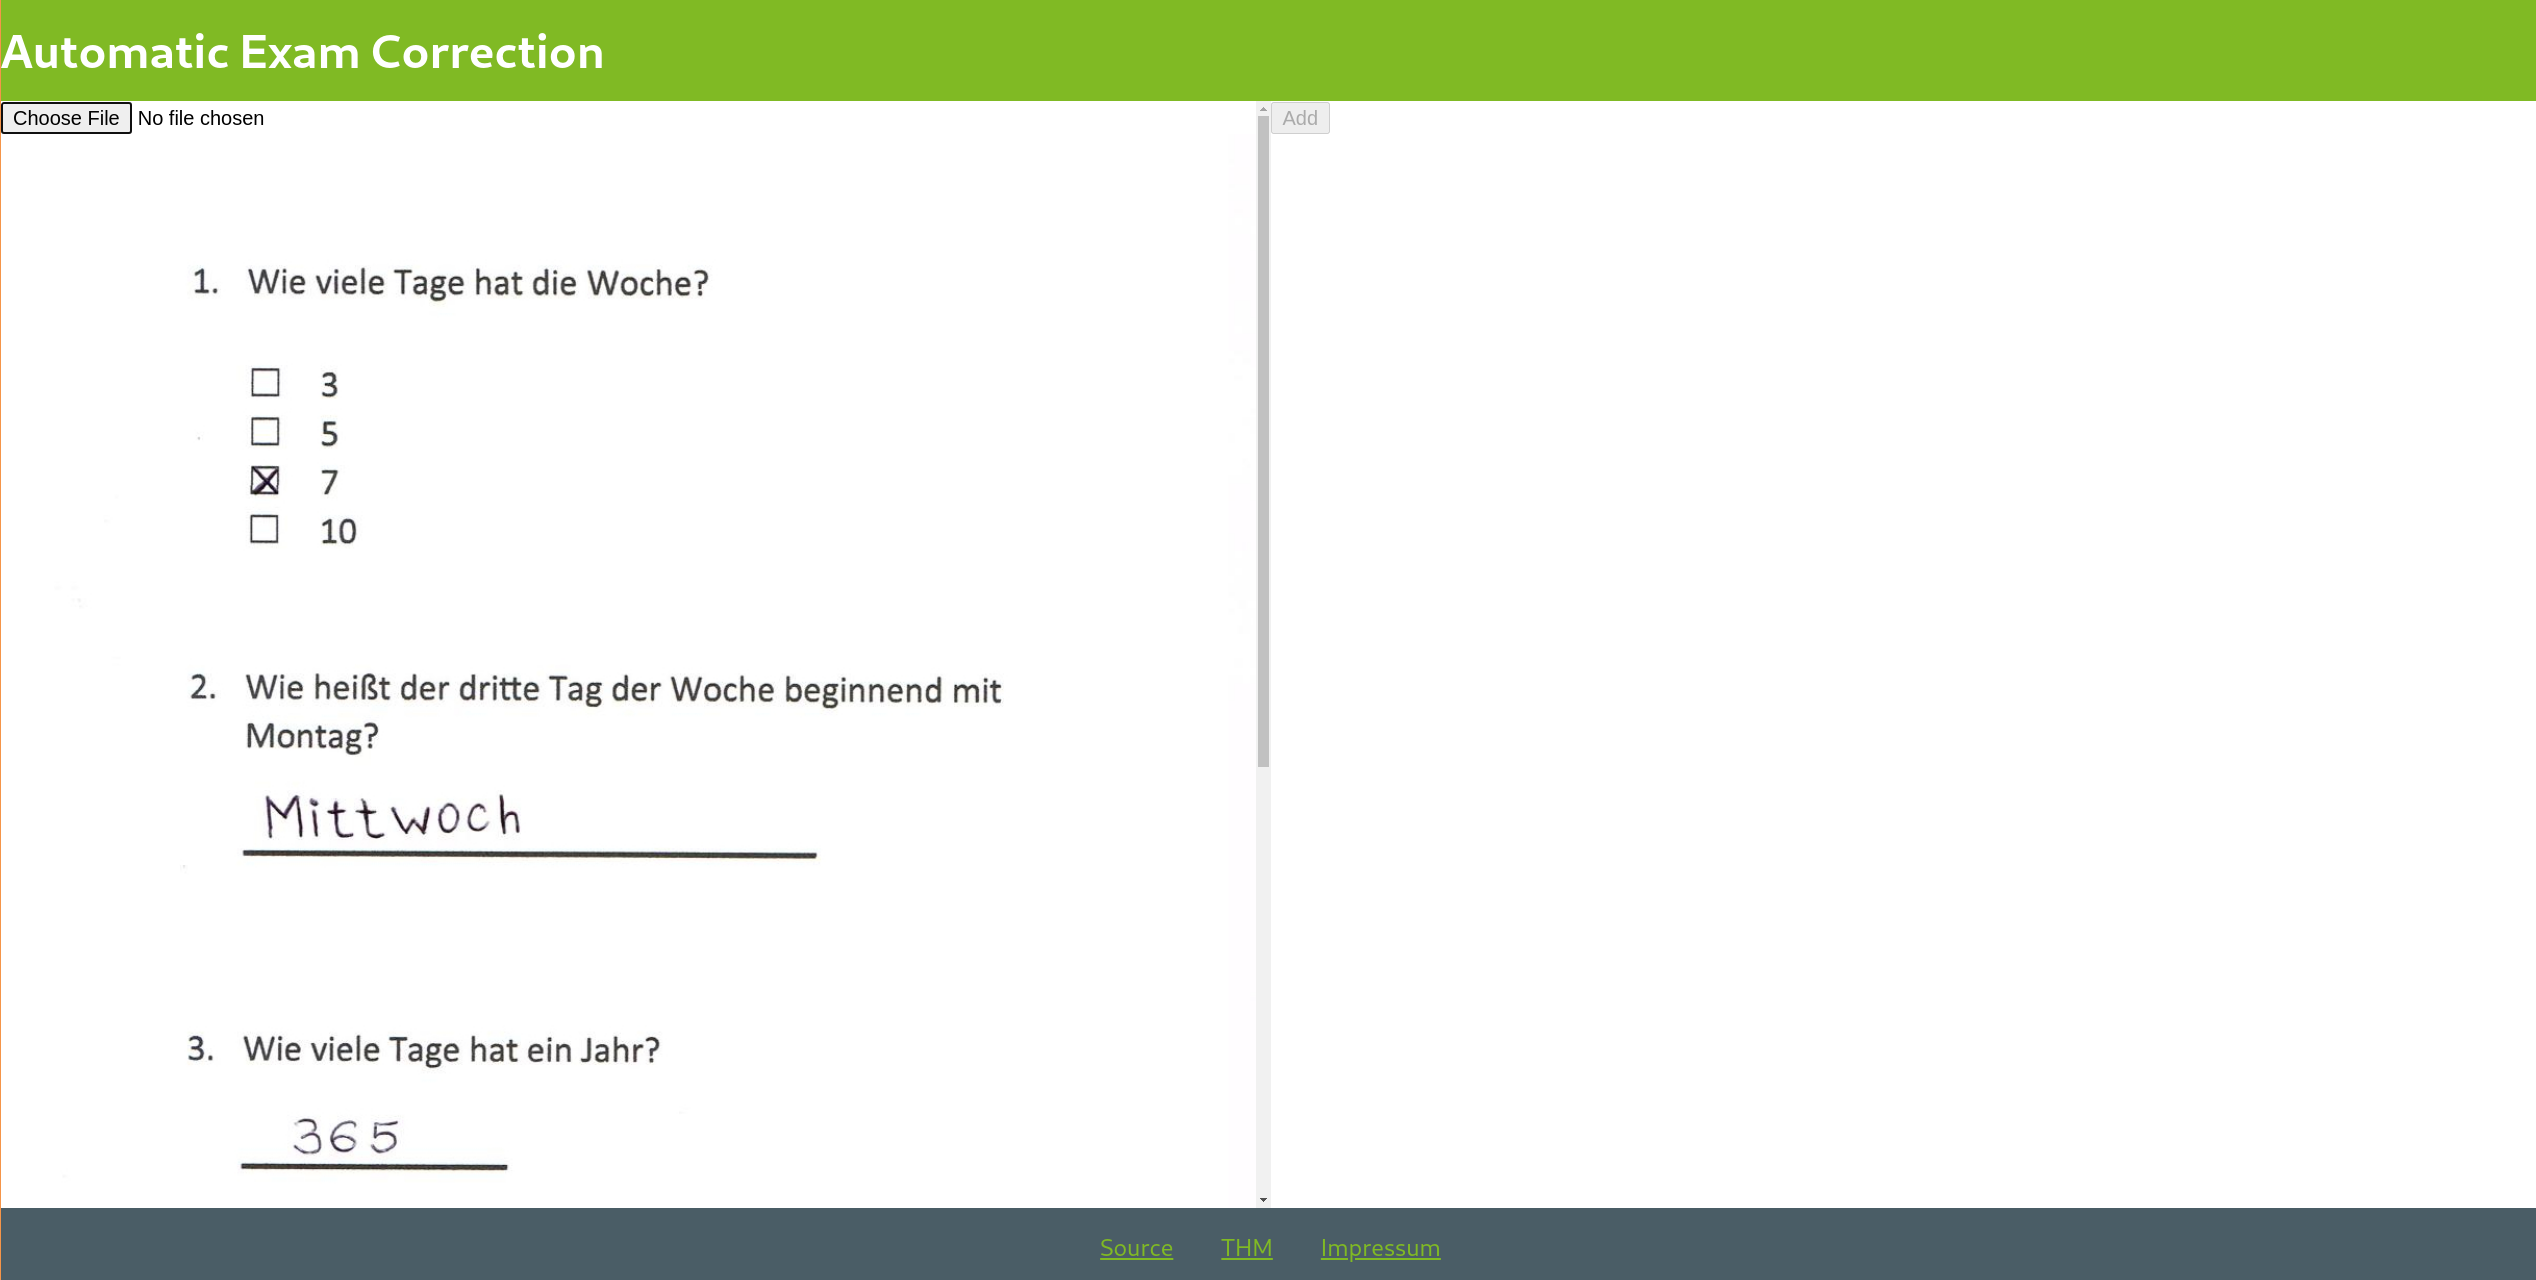
\includegraphics[width=\textwidth]{loaded-muster}

Per Maus kann nun ein Bereich ausgew\"ahlt werden, dabei ist zu beachten, dass dieser etwas Platz l\"asst zwischen dem Markierten Teil der Aufgabe und dem umliegendem Bereich.
Wichtig ist es nur den Teil zu markieren in dem auch eine Antwort erwartet wird, also nicht die Frage an sich markieren.

Mehr Informationen zu dem Thema "gut markieren" finden Sie in dem Kapitel "Aufgabentypen".

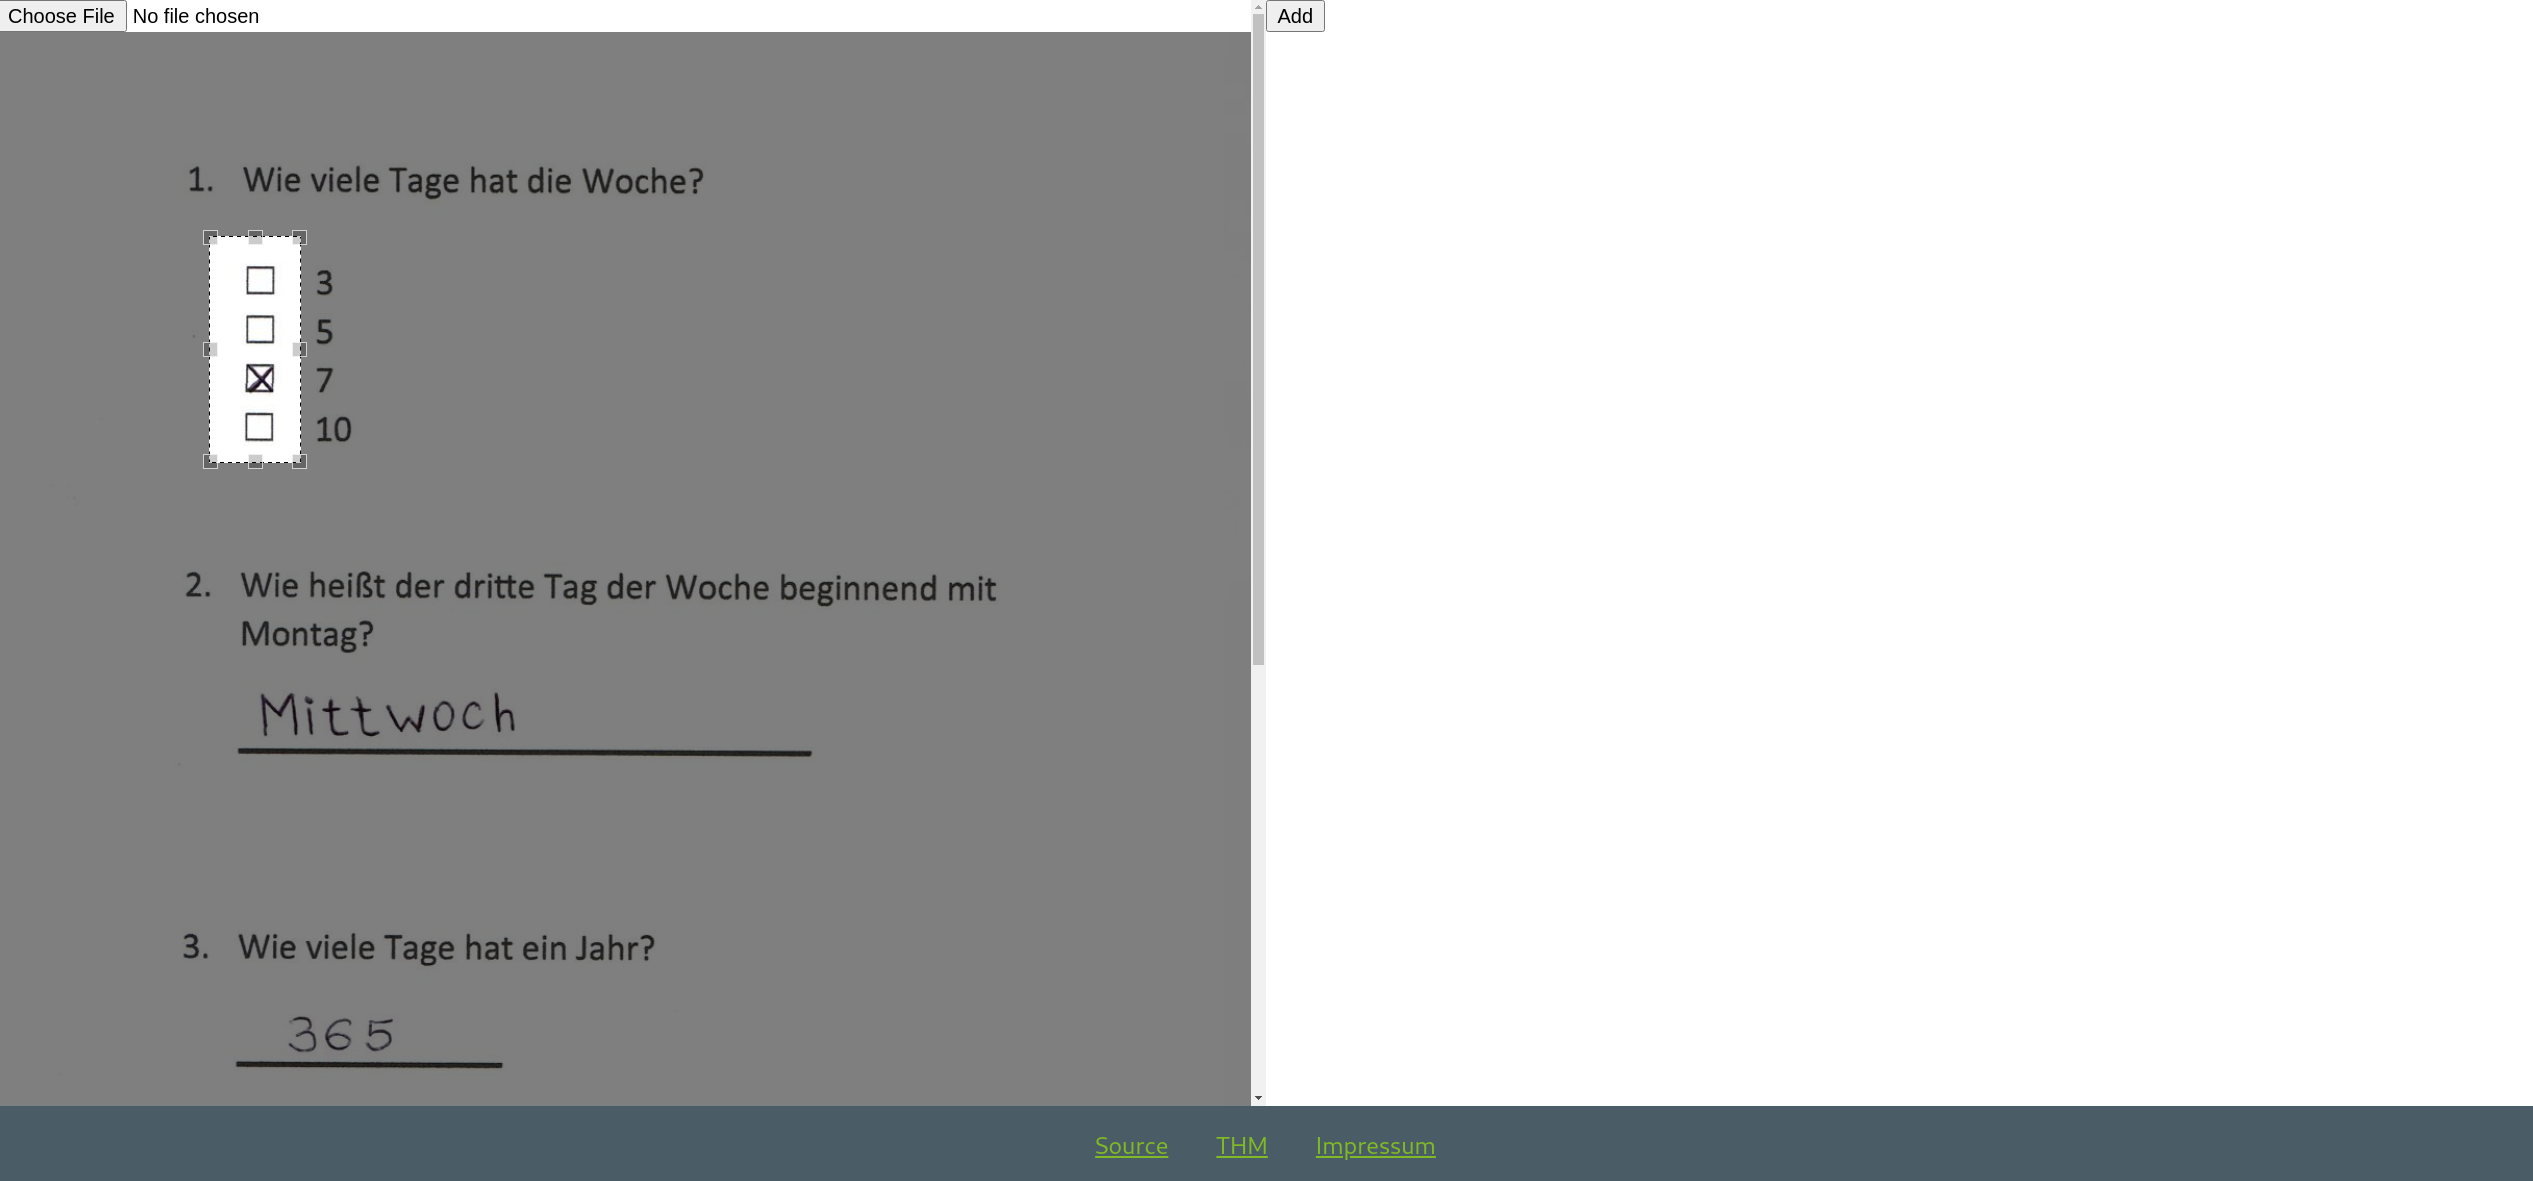
\includegraphics[width=\textwidth]{select-task}

Wenn auf den "Add" Butten geklickt wurde, erscheint folgende Darstellung, hier kann der Aufgabentyp, die maximalen Punkte und der Abzug pro Fehler gesetzt werden.
So kann mit dem Button "Delete" auch die Auswahl gel\"oscht werden und mit dem Button "Edit" der ausgew\"ahlte Bereich ver\"andert werden.

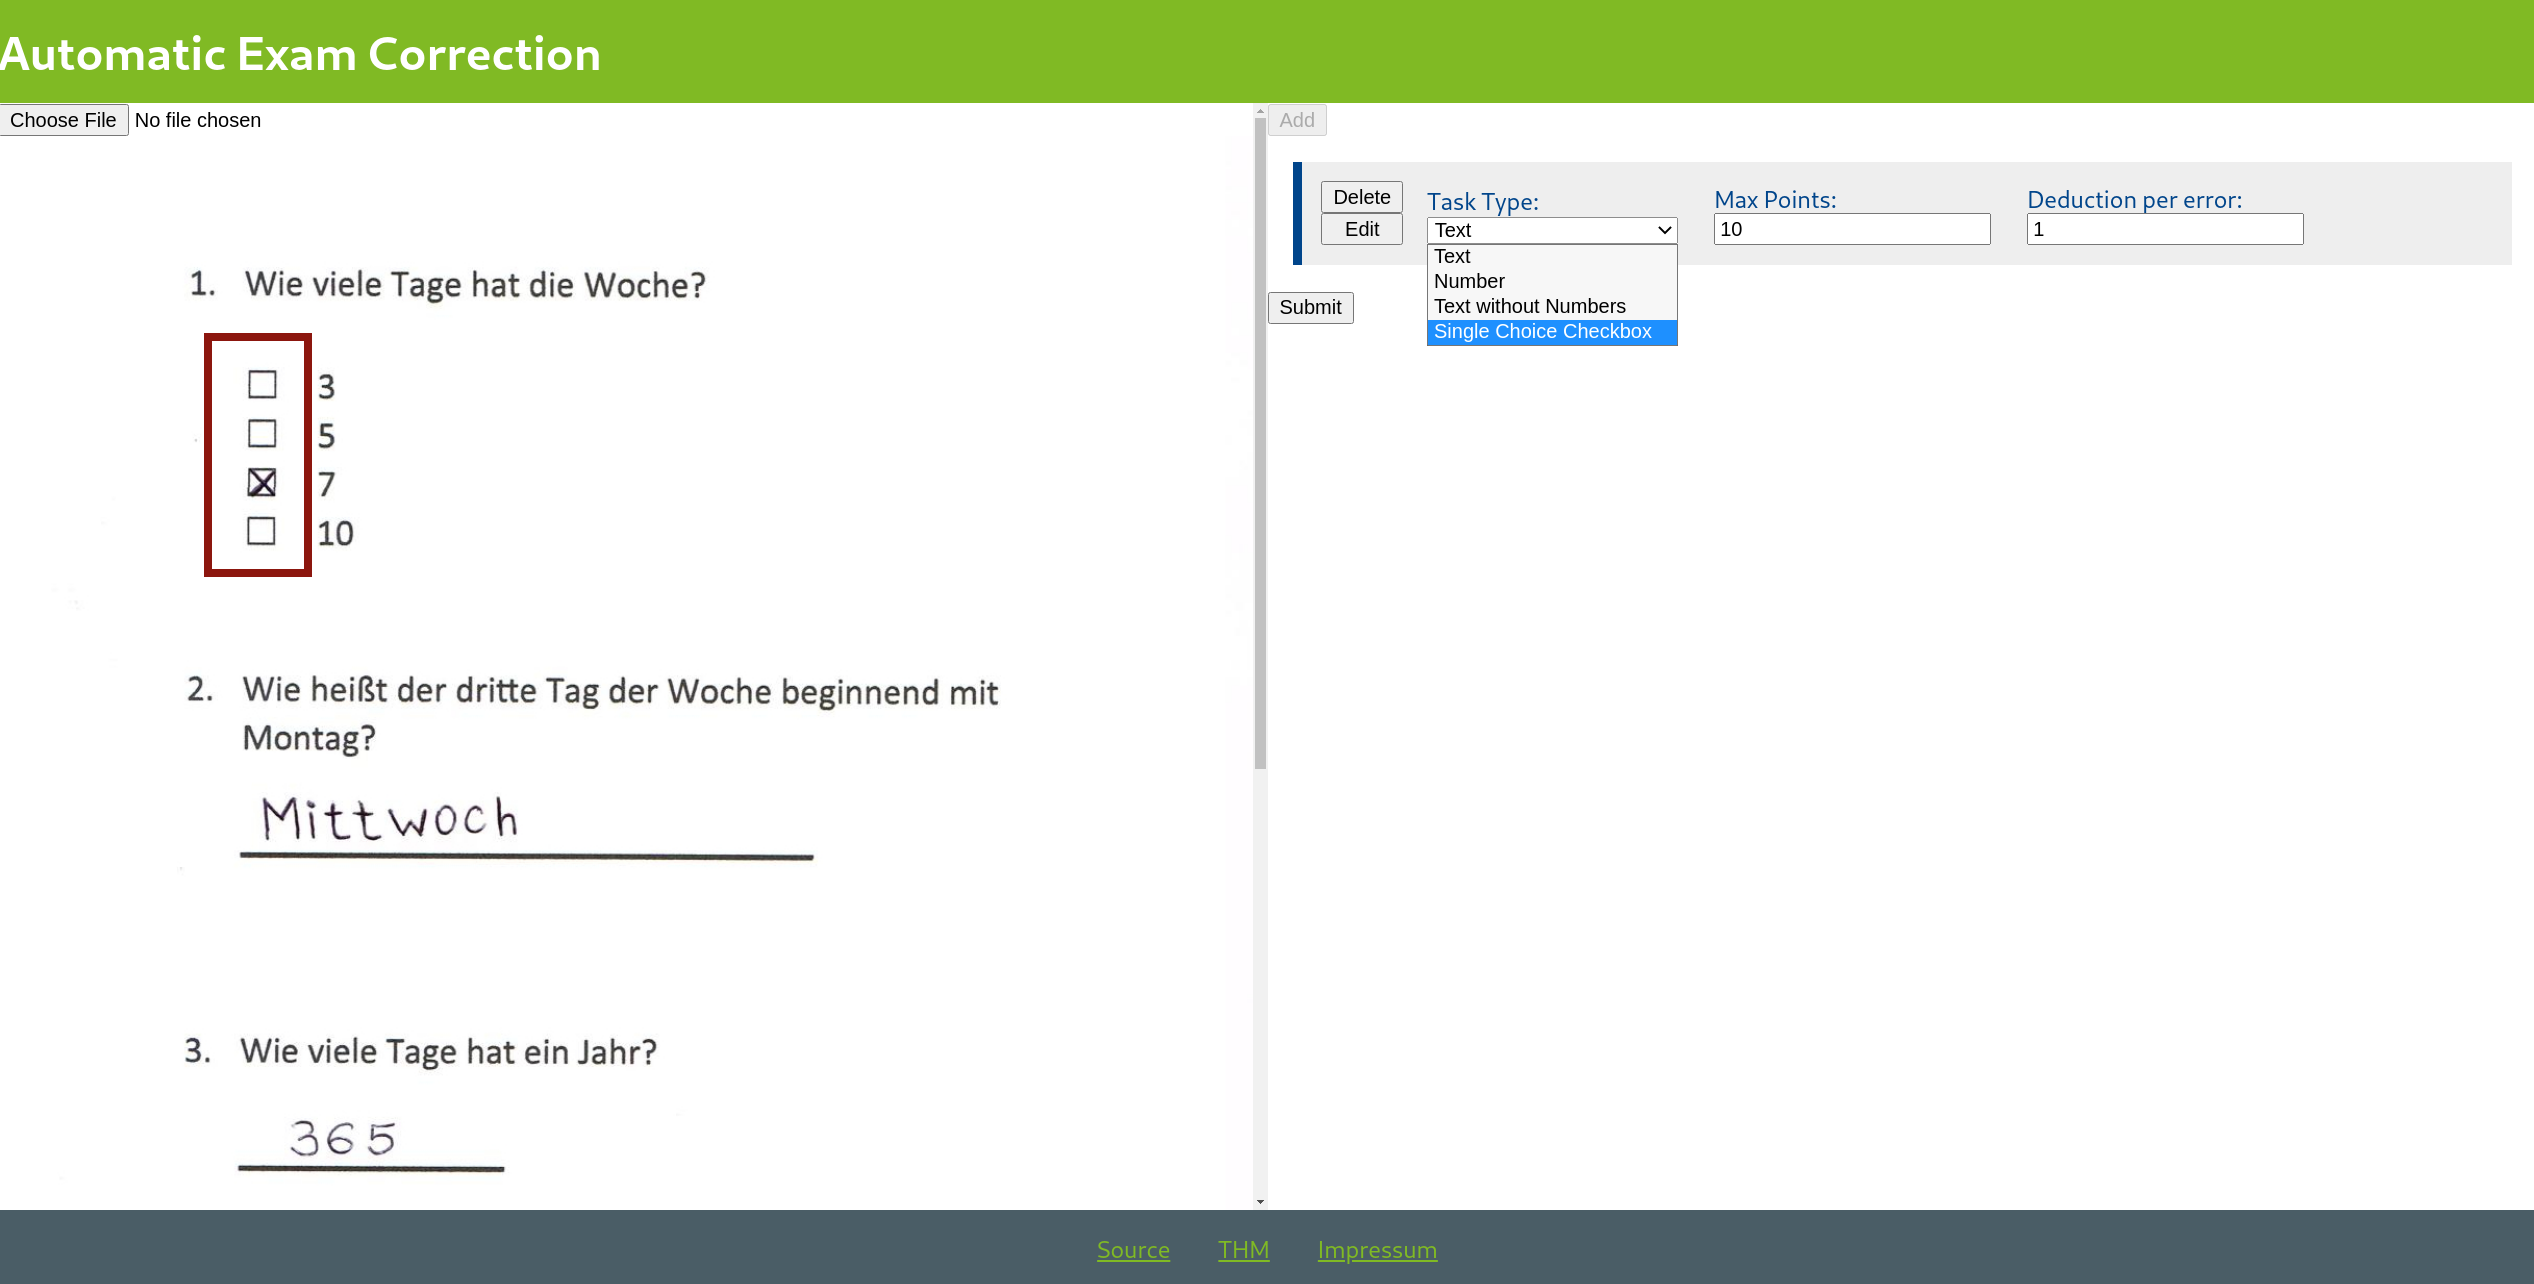
\includegraphics[width=\textwidth]{select-task-type}

In der diesem Bild sind nun mehrere Aufgaben gew\"ahlt.
Es ist hier besonders zu beachten die Aufgabentypen "text", "numbers" und "text without numbers" entsprechend zu setzen.
Dies erh\"ot die Genauigkeit der automatischen Erkennung sehr.
Wenn alles nun noch einmal kontorolliert wurde, kann der "Submit" Button gedr\"uckt werden, dadurch werden die ausgew\"ahlten Bereiche automatisch erkannt.

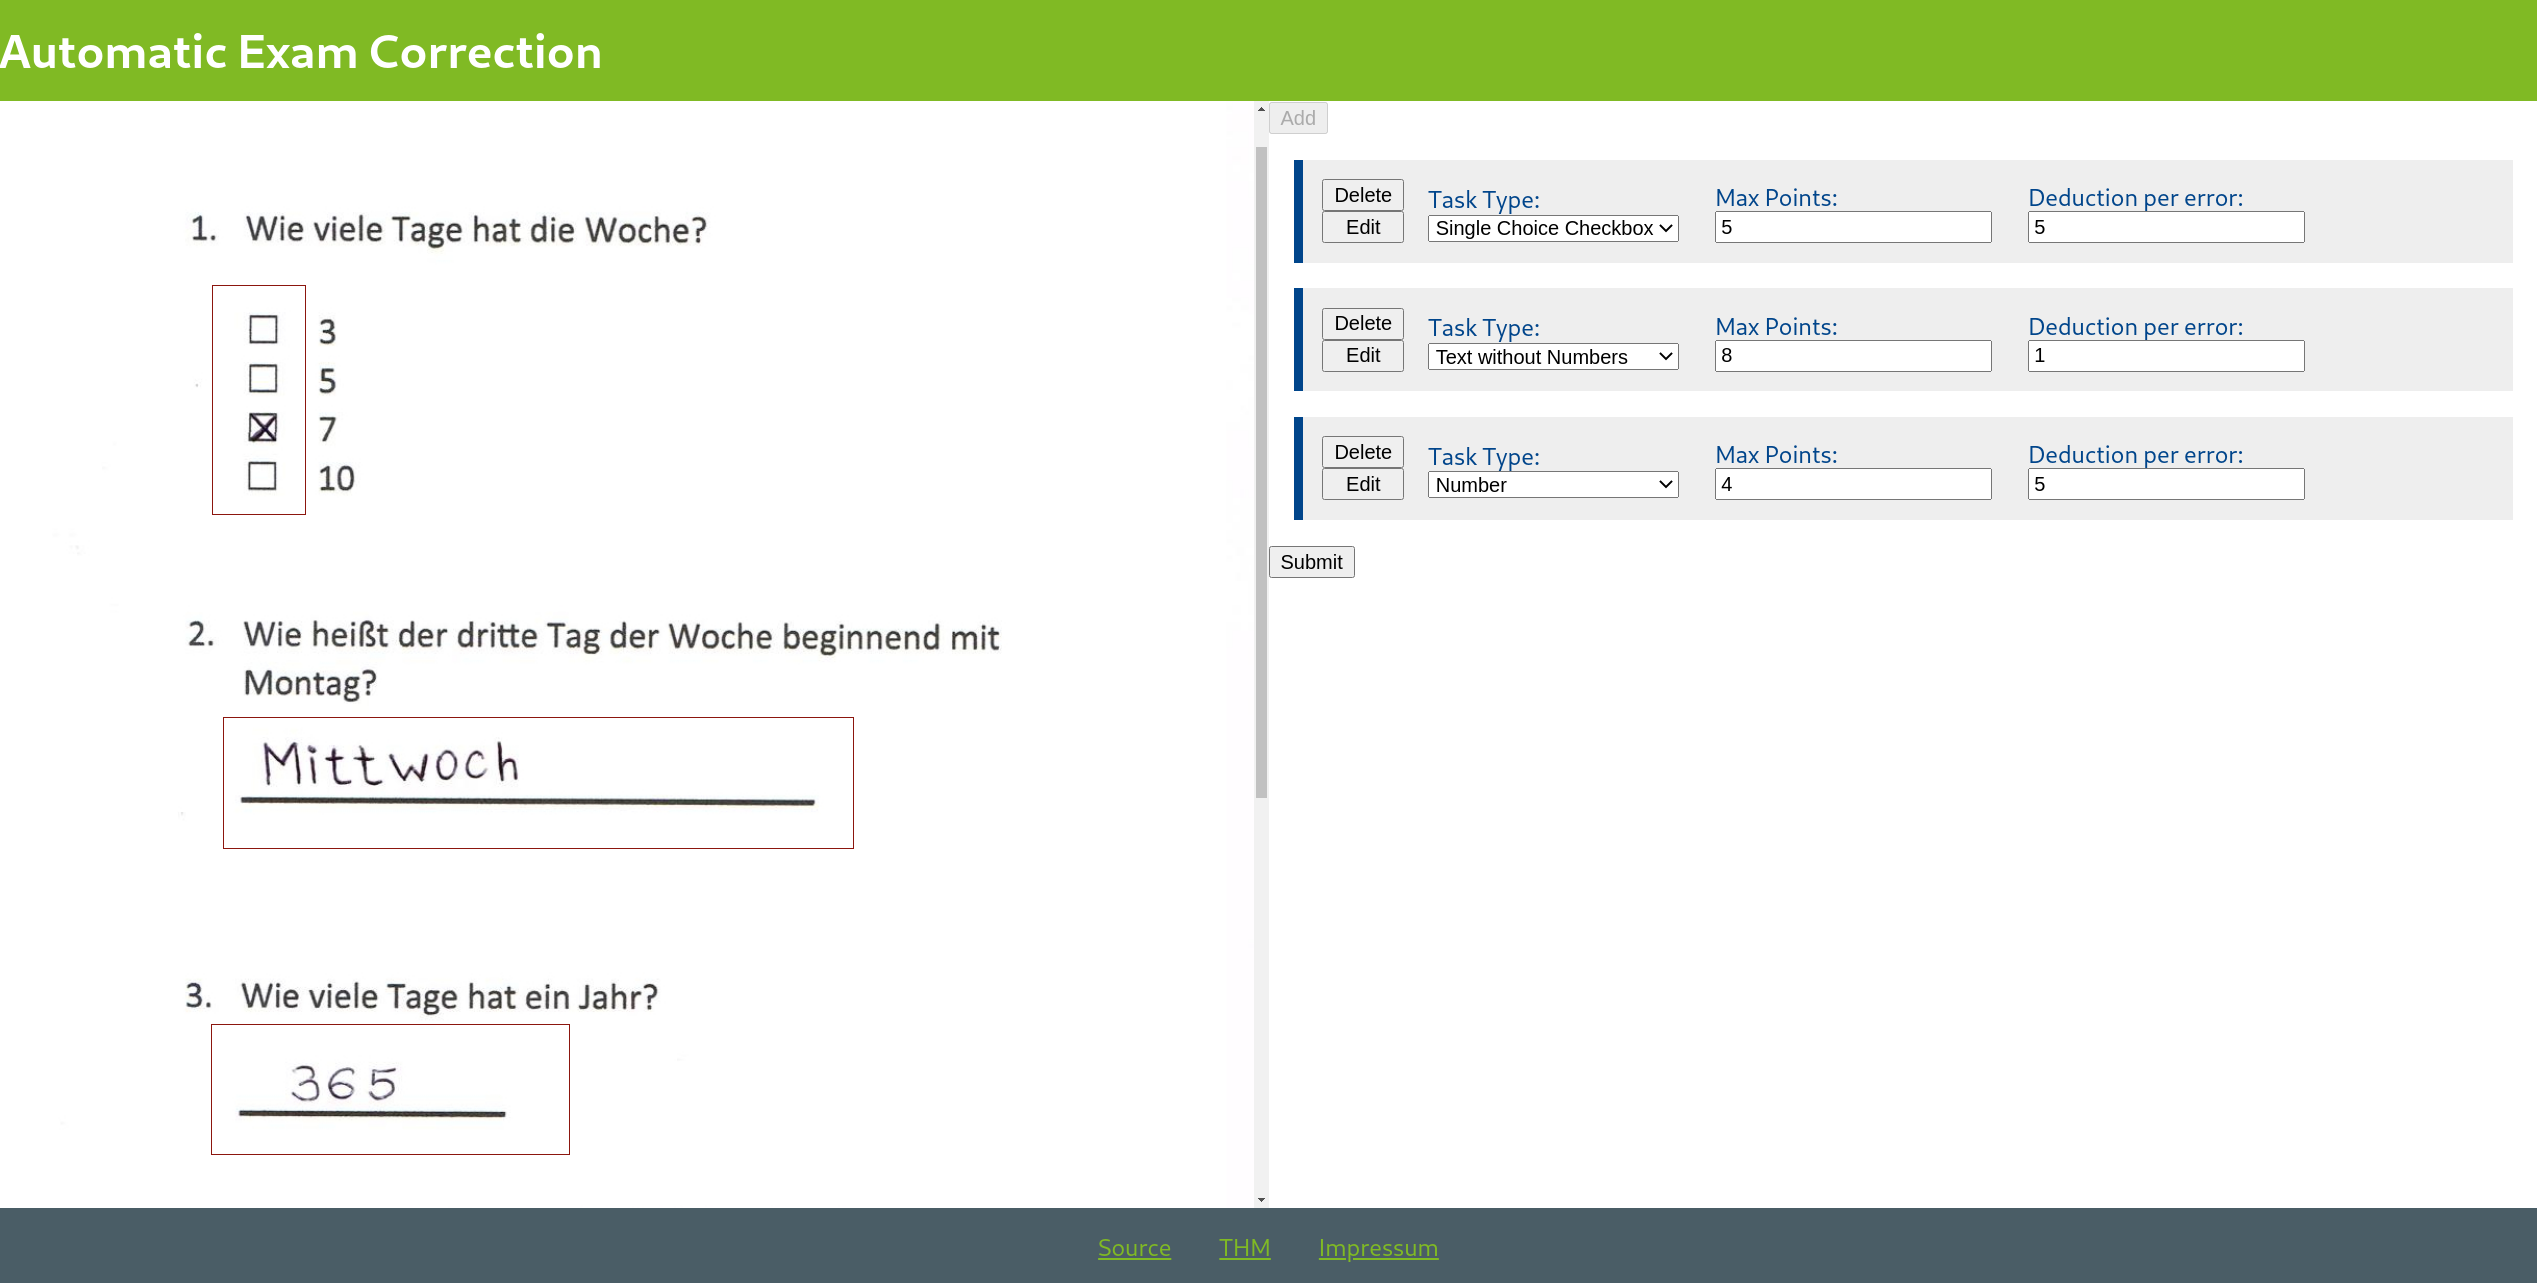
\includegraphics[width=\textwidth]{multiple-tasks-set-points}

\subsection{Erkennung von Musterl\"osung und laden der Formulare}

Es ist wichtig, dass die Erkannten Aufgaben von einem Menschen noch einmal \"uberflogen werden, da die automatische Erkennung nicht immer korrekt ist.
Dazu kann man in der n\"achsten Ansicht einfach auf die Textfelder die mit "Correct Answer" beschrieben sind klicken und dort den korrekten Text eingeben.

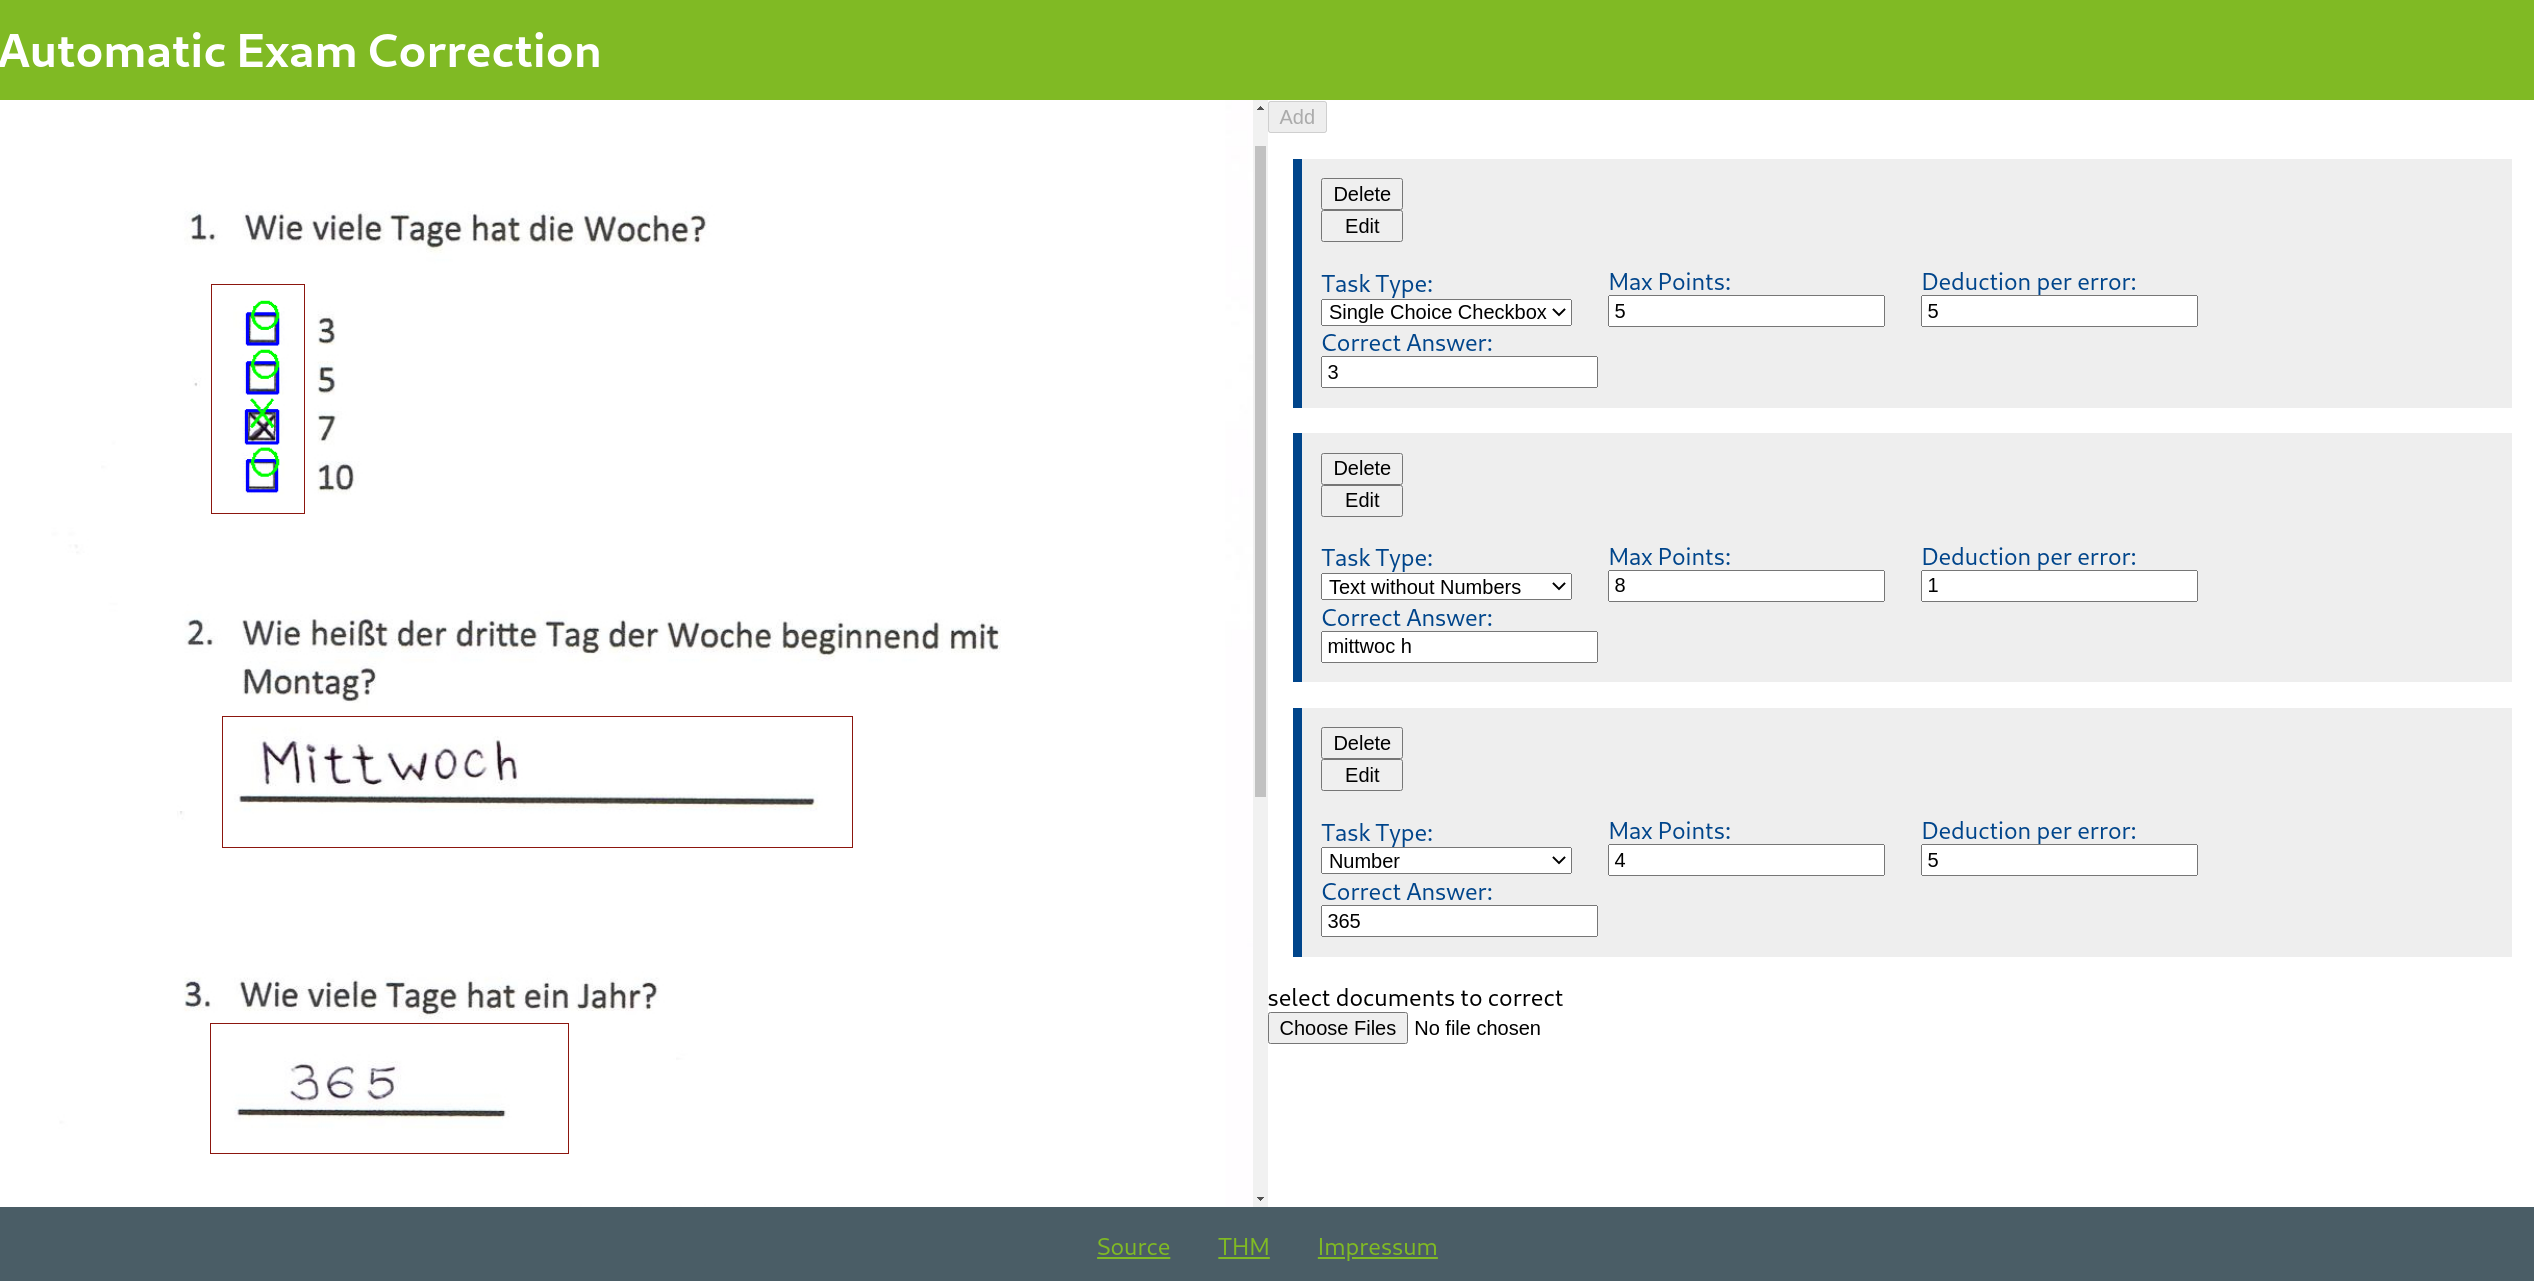
\includegraphics[width=\textwidth]{detected-sample-solition}

Darauf sollten dann die korrekten Anworten gesetzt sein und die gew\"unchten Punktzahlen eingetragen sein.

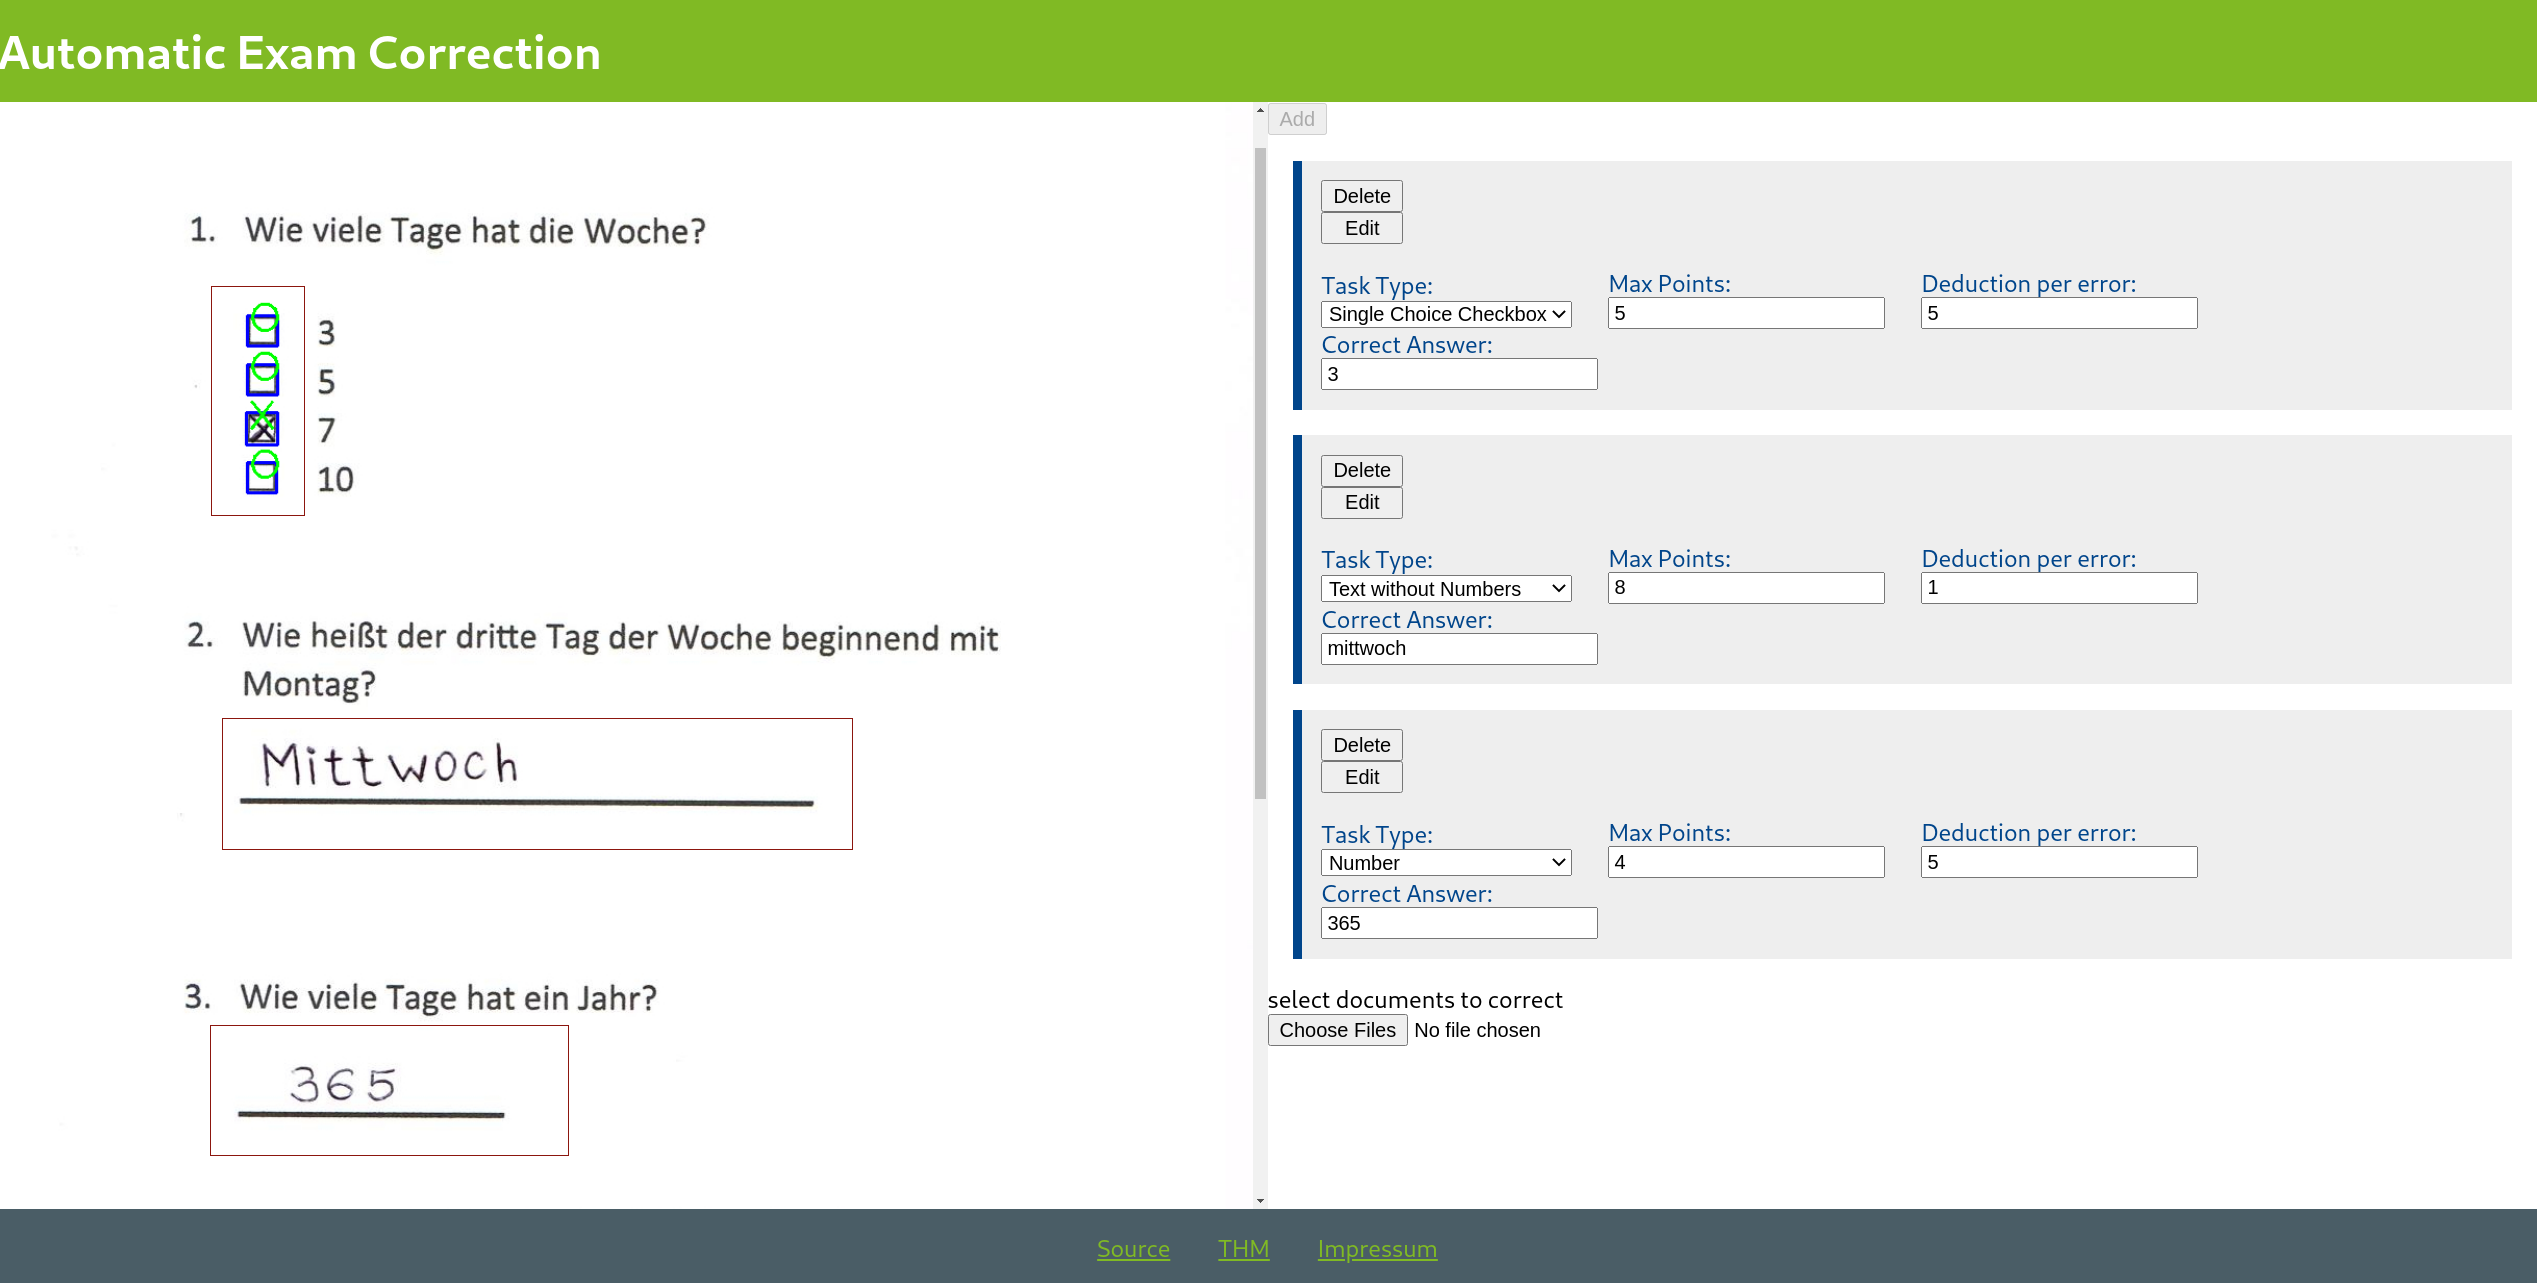
\includegraphics[width=\textwidth]{detected-sample-solition-corrected}

Nun k\"onnen ein oder mehrere zu korrigierende Formulare ausgew\"ahlt werden mit dem Button "Choose Files".
Sobalt dies geschehen ist, erscheint der "Next" Button.

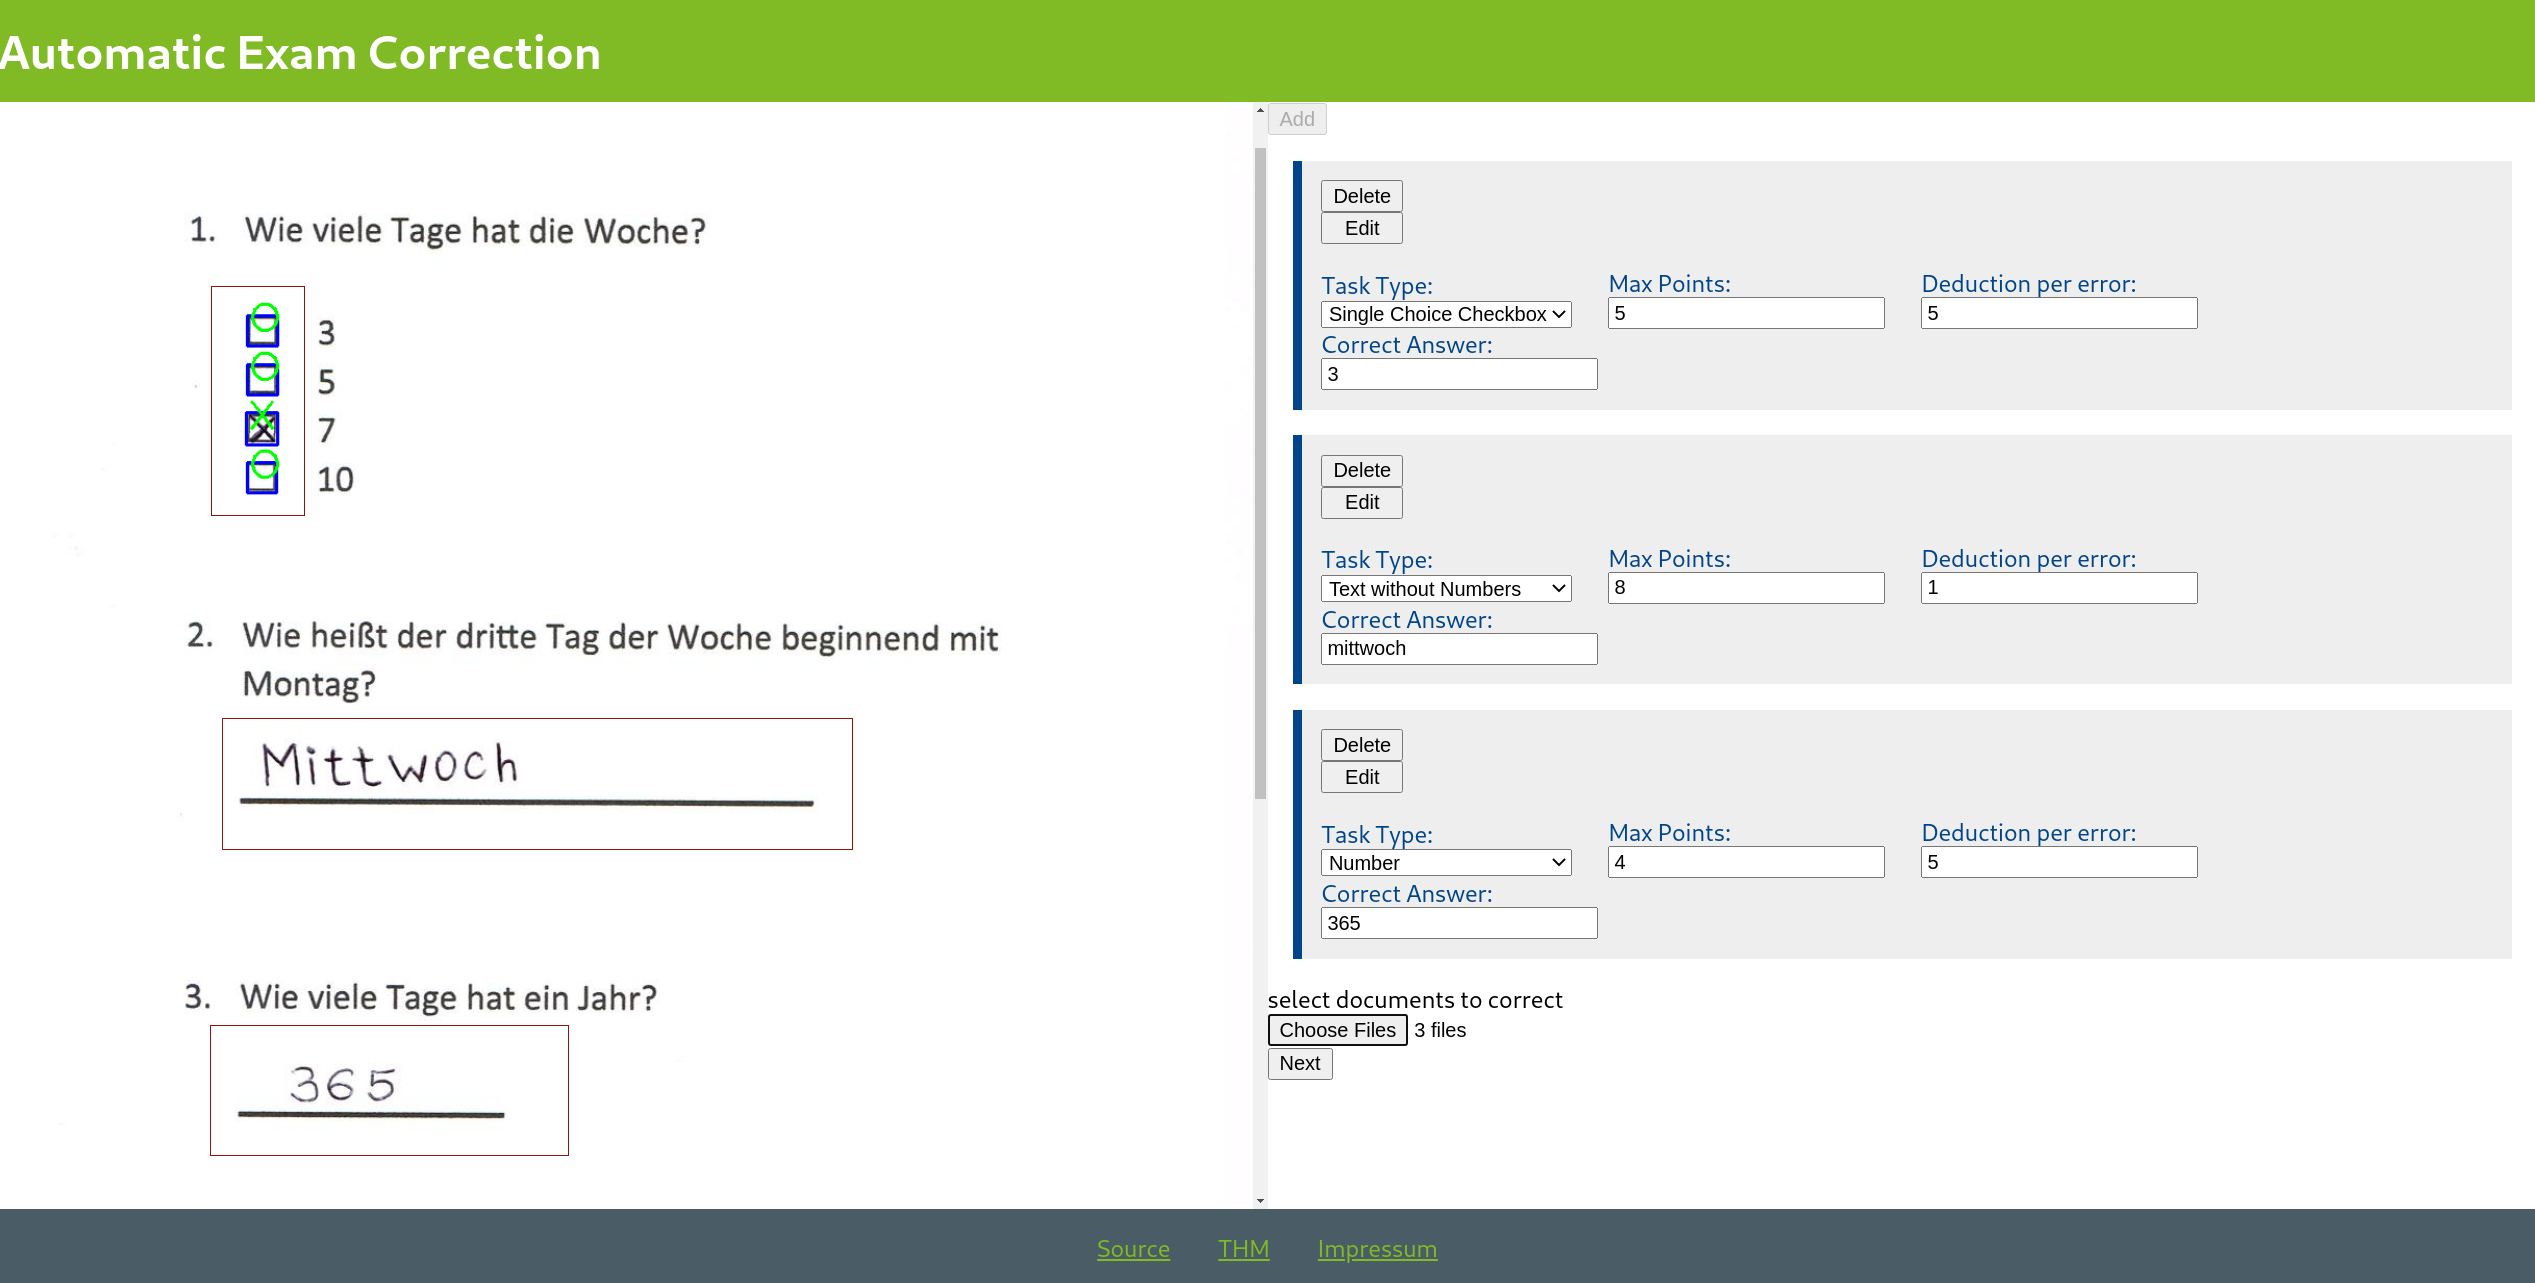
\includegraphics[width=\textwidth]{exams-selected}

\subsection{Korrigierte Fomulare \"Ubersicht und Korrektur}

Nun bekommt man eine \"Ubersicht \"uber alle korrigierte Formulare.
Rechts sind die Durchschnitte der einzelnen Aufgaben zu sehen, w\"ahrend links die einzelnen Formulare zu sehen sind.

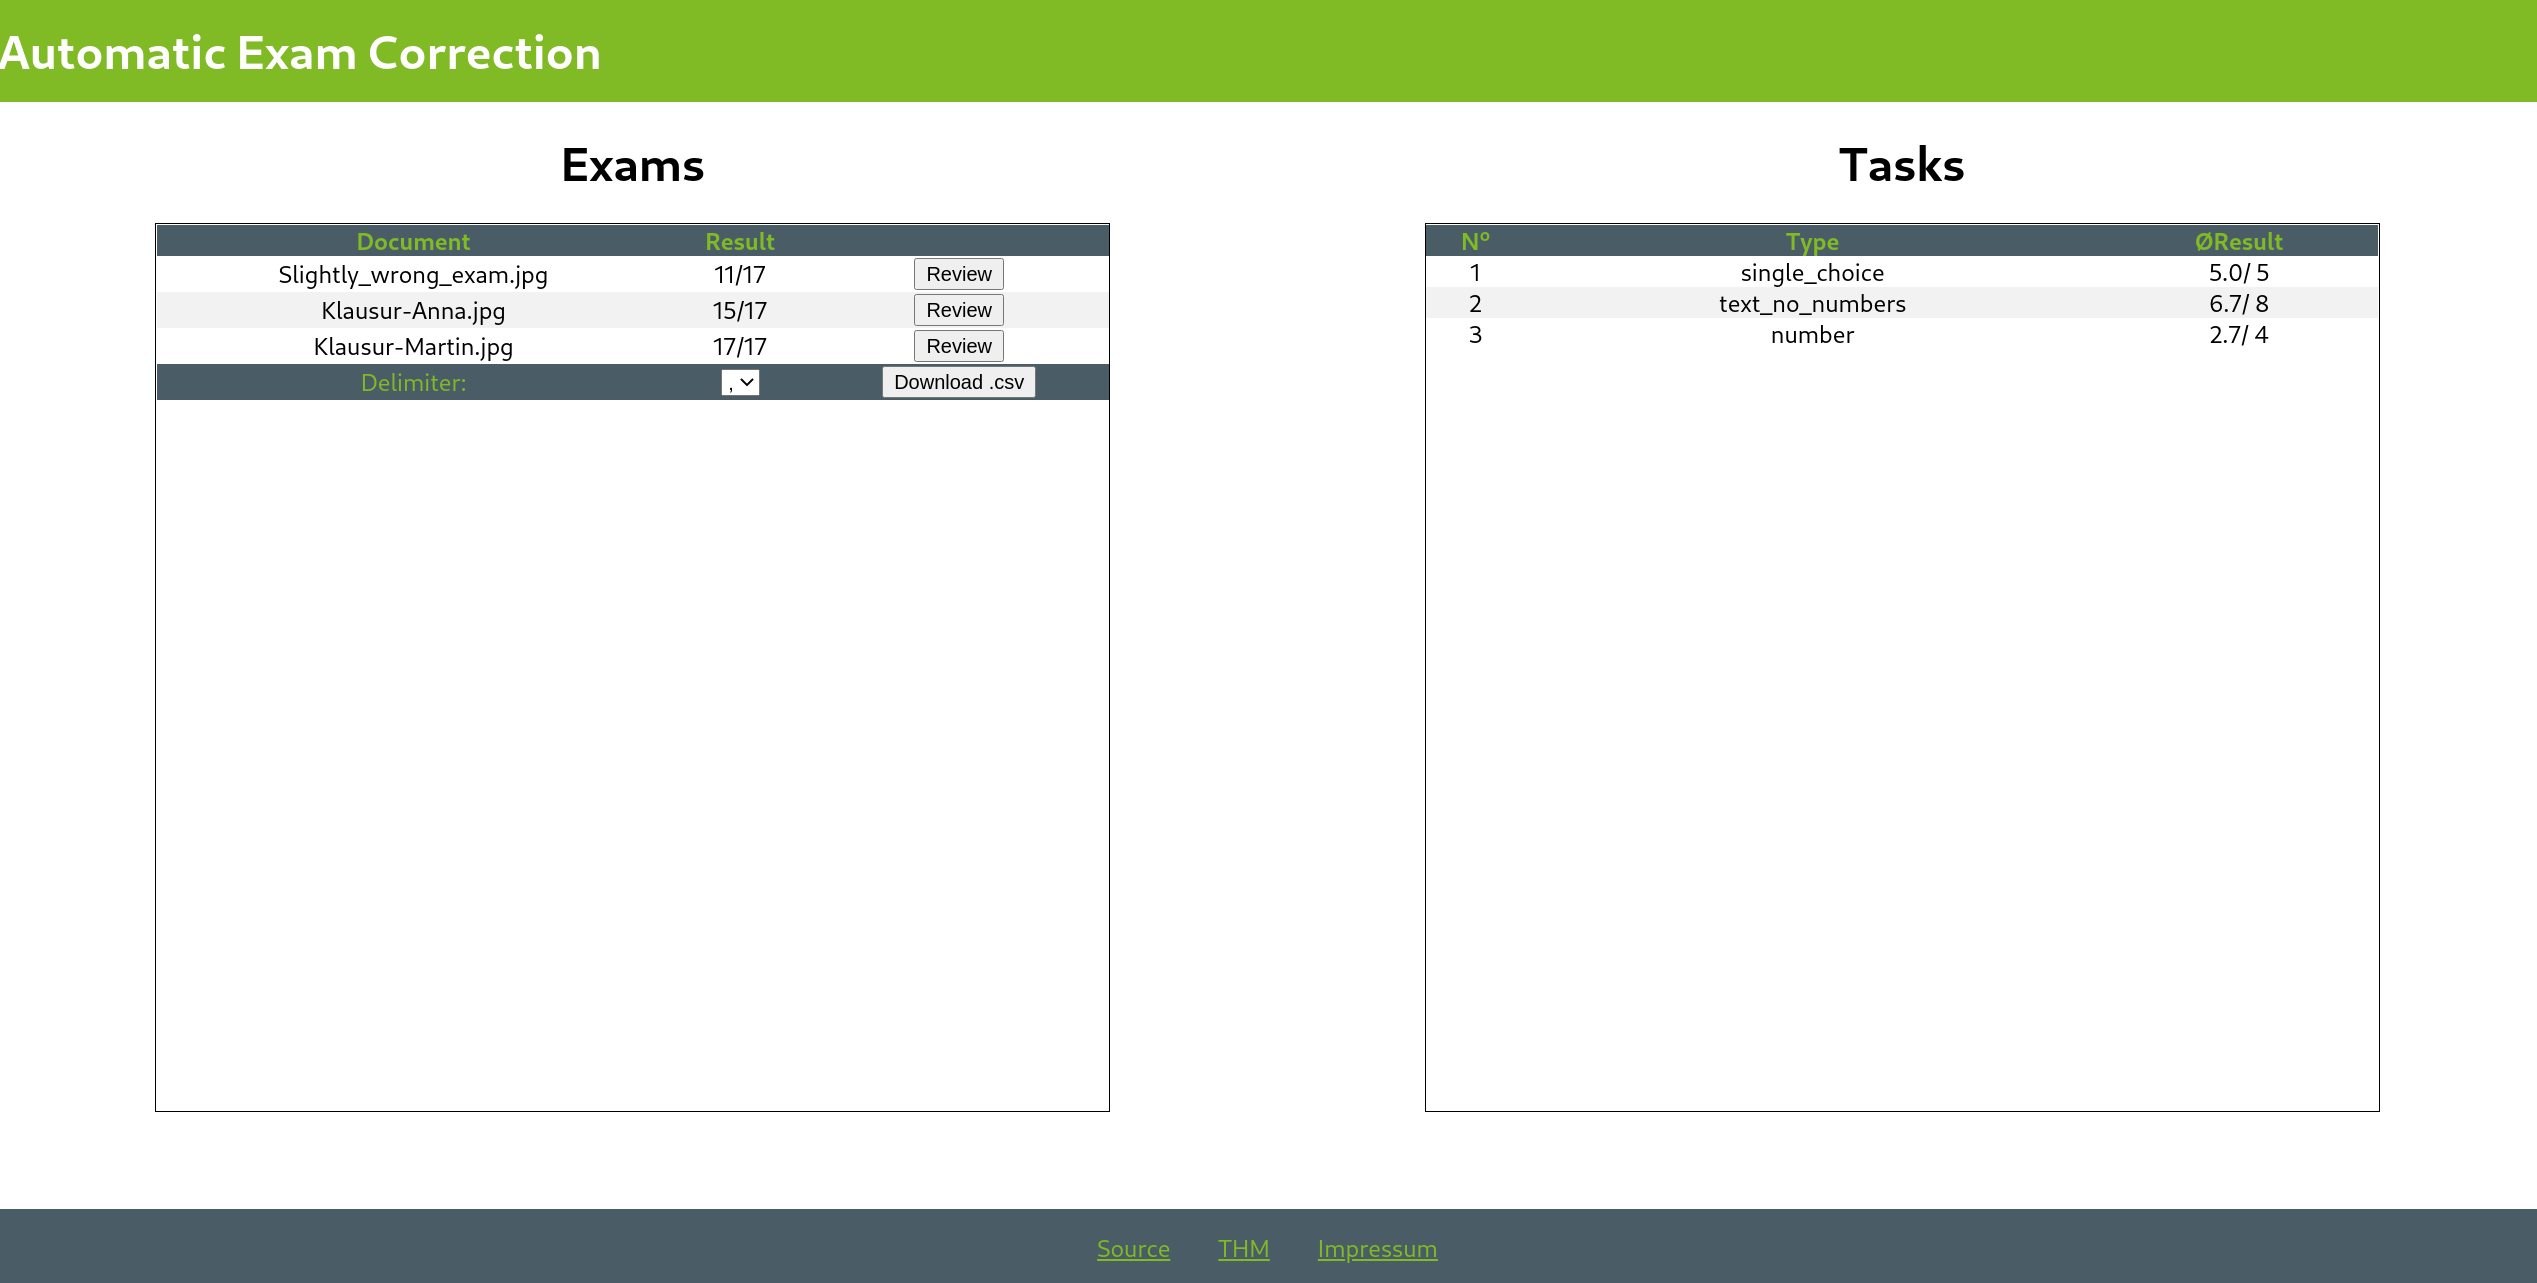
\includegraphics[width=\textwidth]{review-overview}

Wenn auf der linken Seite bei einer der Fomulare auf "Review" geklickt wird, wird das Formular ge\"offnet.
Dort kann dann gepr\"uft werden, ob die Aufgaben korrekt erkannt wurden.
Au{\ss}erdem k\"onnen hier die Punktzahlen der Aufgaben ver\"andert werden.

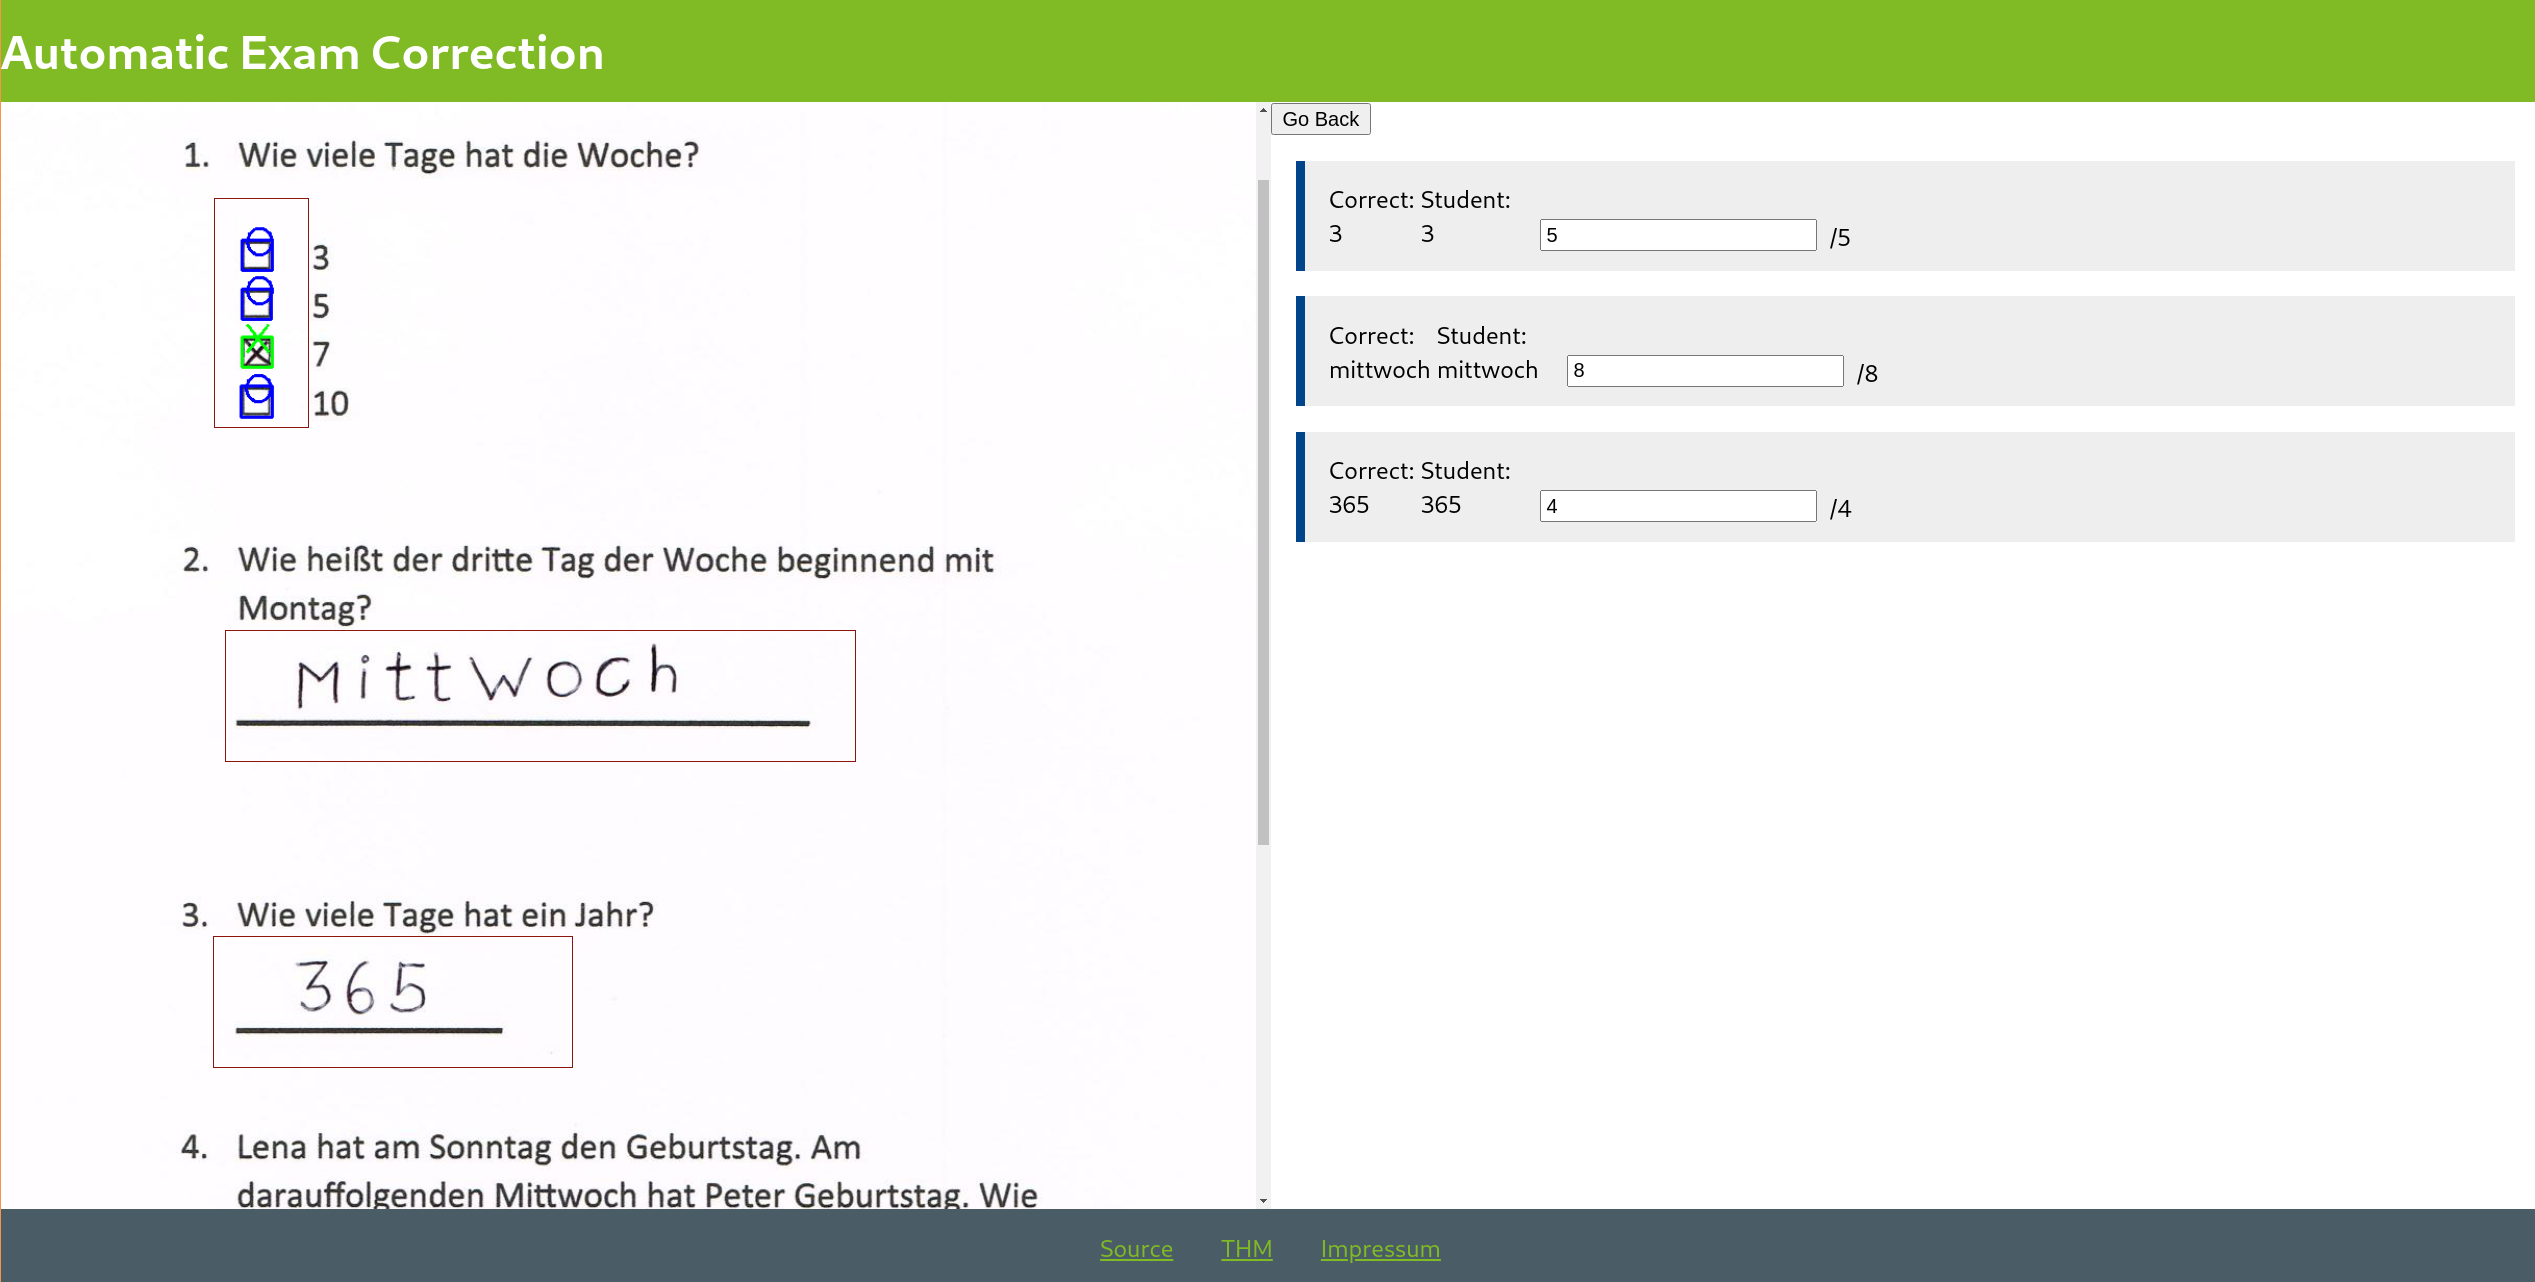
\includegraphics[width=\textwidth]{correct-exam-view}

Wenn die Person, welche das Formular ausgef\"ullt hat Fehler gemacht hat, werden die Punkte auch abgezogen (Aufgabe 3).
Hier kann es zu Fehlern der Software kommen wie in dem folgendem Screenshot sichtbar ist.
Aber sobalt man in dem Formular die Punkte ge\"andert hat, wird das Formular mit der neuen Punktzahl gespeichert.

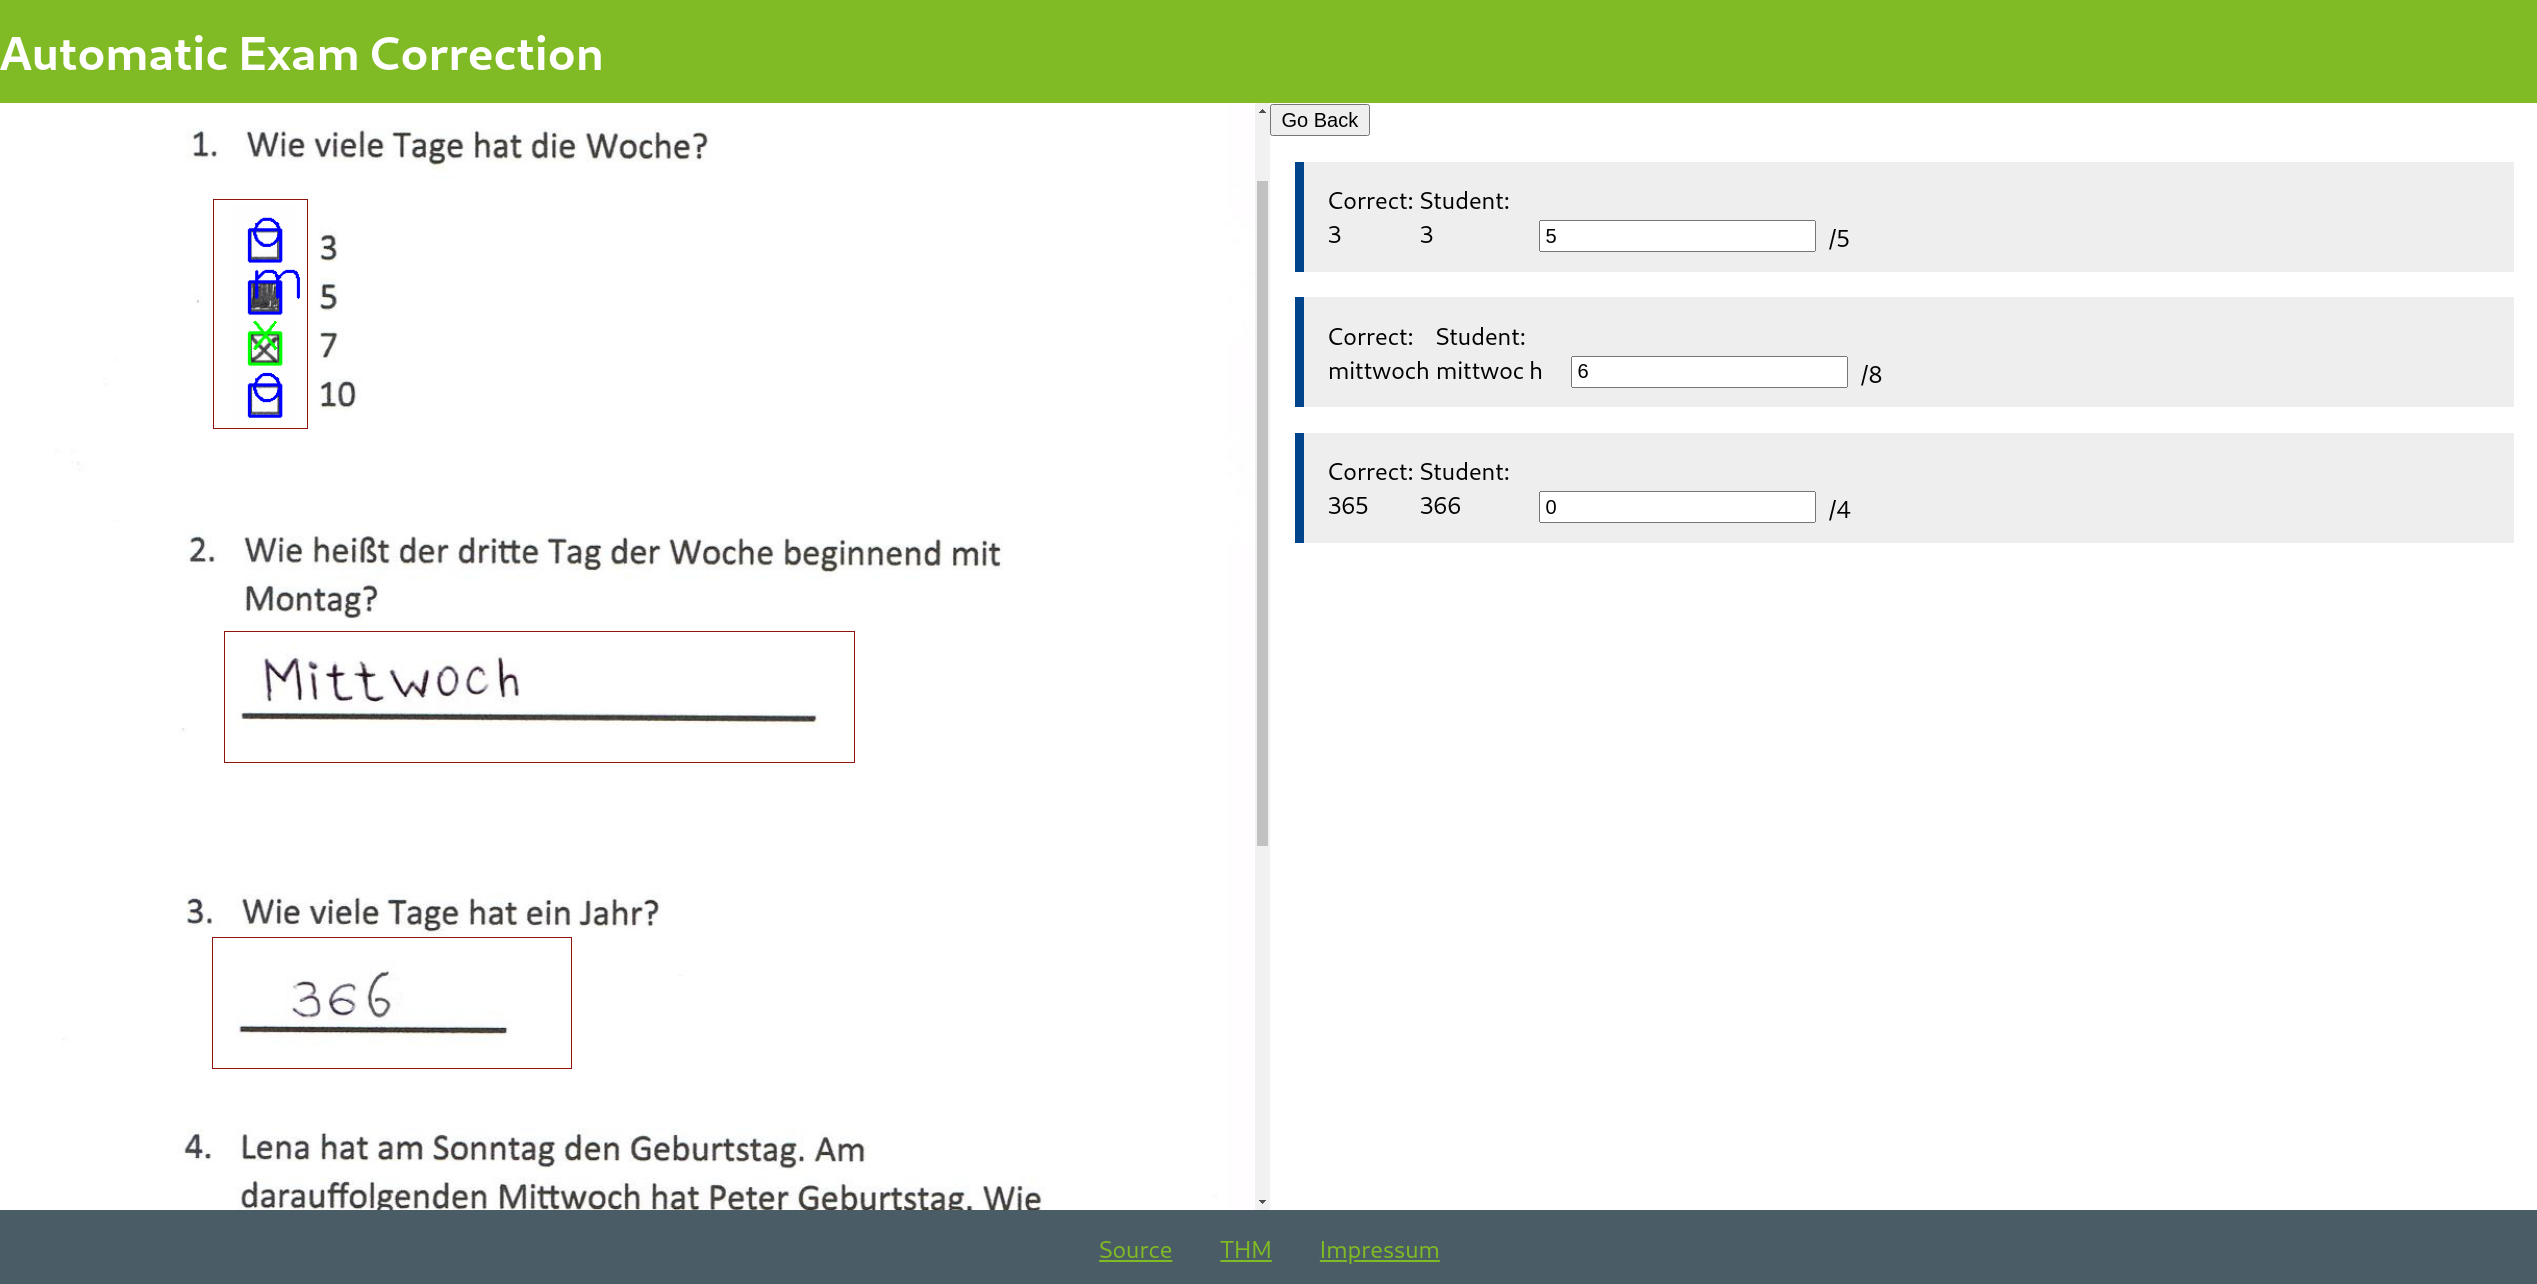
\includegraphics[width=\textwidth]{exam-with-errors}


Abschlie{\ss}end kann man die Punkte noch downloaden als CSV Datei, diese lassen sich leicht in ein Tabellenprogram Importieren.
Dabei nur beachten, dass der Delimiter (das Zeichen zwischen den Werten) der richtigen Sprache entspricht.
Im Deutschen ist dies ein Semicolon: ';'
Im Englichen/Global ist dies ein Komma: ','
